% Este documento contiene el índice del manuscrito de la tesis.
%\documentclass[12pt,a4paper]{report}
%\usepackage{graphicx}
 
%\title{Introduction}
%\author{Claudia Guti\'errez}
%\date{ January 2018}


%\begin{document}

%\maketitle

%\tableofcontents{}

%%%%%%%%%%%%%%%%%%%%%%%%%%%%%%%%%%%%%%%%%%%%%%%%%%%%%%%%%%%%%%%%%%%%%%%%%%%%%%%%%%%%%%
\part{Introduction\label{cha:intro}}

\chapter{Context and introduction\label{context}}

% \epigraphfontsize{\small\itshape}
% \epigraph{''Begin at the beginning,'' the King said gravely, ''and go on till you
% come to the end: then stop.''}{--- \textup{Lewis Carroll}, Alice in Wonderland}

\section{A changing world} 

% Ideas a desarrollar:

% * Un mundo en constante evolución.
% * Cambio climático
% * Transición energética global
% * Cambios sociales/políticos.
% * Migraciones

It is said that nothing is permanent except for change. We are in a constantly evolving world where, unavoidably, some of these changes will go over us without us  being able to adapt to them. Meanwhile, other changes will go unnoticed because of their slowness or because they are not part of our main concerns. It seems paradox to think that some of those human induced changes, consciously or unconsciously, willingly or by mistake, will make human beings resist an get adapted as a species against the consequences of something that they themselves created. 

The evolution and development of nations has been linked since the first Industrial Revolution to an increment on the energy demand. The use of fossil fuels since the vapor engine has changed the well-being of societies. Related to this increase, the green house gasses (GHG) emissions and their concentration in the atmosphere has risen dramatically in contrast to pre-Industrial times. Global warming, with its origin in human activities, is one of the biggest challenges of adaptation for human beings. The \textit{anisotropic} character of the associated impacts of climate change puts our solidarity with the most vulnerable and less responsible communities on trial.

Some people believe we are in what has been described as the Third Industrial Revolution \cite*{Rifkin2012}, a process of exponential scientific-technological development, characterized as a convergence of the evolution of renewable energy technologies and the massive use of new communication technologies. The ongoing energy transition should be the answer to committed citizens that find those technologies as an alternative and an answer to the environmental challenges and associated consequences.     

The actual context is characterized by an advanced globalization where the borders have been blurred through telecommunications development and international migration movements are becoming more feasible. In 2015, there were 100 millions more people living in a different country of its birth country than in 1990 [International Organization for Migration]. Most of that movements are related to work opportunities or family issues. However, the increase of the population and the rising demand of natural resources to support a system based on the continuous growth lead to geopolitic conflicts and the depletion of natural resources \cite*{Rosa2012,commoner1991}, what supposes an increase in migration movements of different character. Populations migrate away from conflict areas or most affected areas by natural disasters [ref ``Environmental Migration Portal'', ref ``International Organization for Migration'']. In that sense, these movements affect most vulnerable people and require special attention.

In order to address the human needs in a juncture of population growth, increase of energy demand and environmental crisis, a paradigm shift is needed. This change would mean recognizing our interdependence with every ecosystem and all living beings as well as recognizing the importance of nature itself. In 1962, Thomas Kuhn wrote in his book  "The Structure of Scientific Revolutions" that a paradigm shift does not occur until the adherents of the old paradigm are replaced with the new generation. We should then wait to see the end of this paradigm shift hoping that it is not too late.

\section{Renewable Energy}

%\subsection{Concept of energy}

% The physics concept of \textbf{energy} is defined as the capacity of a system to perform a work and it is divided into two groups: kinetic energy, that is related to the movement of the system, and the potential energy, related to its position. For this fundamental classification, mechanical energy, electromagnetic and thermal energy are encompassed in the kinetic energy group, while the chemical energy or the gravitational potential energy, as it is the case of hydropower,  are inside the potential energy group.
 
% \subsection{Types and classification}

% It is elementary to delimit the differences between kinds and sources of energy. Sources of energy are defined as those from which useful energy can be extracted, and directly applied to its purpose (being this one movement, electricity production or metabolic processes) or by undergoing any transformation process.

In the context of society's energy consumption we call \textbf{primary energy sources} those from whom, after a process of extraction or transformation and transport, we are able to obtain final energy to be used. Regarding that, we consider fossil fuels as a primary energy source, as well as hydro-power, solar energy or biomass. %These sources of primary energy provide the final energy that many times will be in the form of electricity. 

These primary energy sources can be classified depending on their origin, being \textbf{renewable} those ones that are inexhaustible. The sun, despite of its unquestionable finite is considered inexhaustible as well, because of the difference in the temporal scale of  human existence and the life of such star, which is lots of magnitude orders above.

\subsection{History and evolution}

The use of renewable energy has come along the development of humanity since ancient times. From the use of biomass to get thermal energy to the transformation of wind energy into mechanical energy to be used in the traditional windmills or for shipping. It was around the middle of the 19Th century with the invention of the vapor engine that fossil fuels started to be used massively and linked to that, what was called the \textit{First Industrial Revolution}. This period meant a big technological development that directly impacted positively on the society's  well being, at least to those from the richest or western countries.

This economic development brought about an increase on the fossil fuels demand that grew up exponentially during the 20Th century. Societies were more and more dependent on energy and evolved turning a blind eye to the reality that the base of their development are finite resources unequally distributed around the globe.

The first step to diversify sources of primary energy did not take place until the 70's, with the first petroleum crisis in 1973 (and the second crisis in 1979) \cite*{Sorensen1991}. The embargo of the petroleum producer countries had some important economic consequences on the importer ones, resulting in the fact that some of them started to consider new sources of energy in order to ensure stability and supply.

In the last decades, in addition to the socio-economic and geopolitic factors that have led to the need of limiting petroleum dependence from importer countries, the stimulus for the big increase of these alternative technologies, has come about due to their decreasing costs, which have the origin in the promotion of support policies. These policies have been driven by different organisms and governments that have created a virtuous cycle around these technologies. The decrease in costs thanks to the support and long-term view policies favors, at the same time, more national target commitments in the use of renewable energy to reduce GHG emissions and to fight against Climate Change. In 2017 more than 170 countries had established goals of renewable generation (IRENA2017).
 
In the actual context, the global energy demand is growing based on the needs of developing countries. It has been estimated that for 2040 it will be up by more than a quarter and it will have an associated shift from Europe to Asia, which will account for 40$\%$ of the energy demand (leaded by China) by that time [WEO2018].

Energy systems accounts for approximately 3/5 of all anthropogenic green house gas emissions [ref] which force us to find the way for a sustainable development that is able to afford human needs. This, unavoidably needs a decarbonization scenario for next years.  

In 2018 renewable energies account for the 18.2$\%$ of the \textbf{final energy consumption} according to the REN21 report [ref], with a share of 27$\%$ in heat generation and $25\%$ for electricity generation. Transport remains the sector with less share of renewable energies with only a $3\%$. These numbers, reflect that contribution of RE to the mix is continuously growing, with increasing relevance in the electricity sector.

Future scenarios continue to project an increase in the energy demand with an overall decrease of the fossil fuel's share. At the same time, it is expected that the power sector increase its share in the final energy consumption distribution. According to that, renewable energies and specially solar and wind are key for delivering low carbon electricity [WEMC].

In 2017, the renewable capacity added was about 178 GW, accounting for the first time for more than 2/3 of global net electricity capacity growth and it was the PV the one that expanded the most with 97 GW [IEA].

%It has been reported that the integration of big shares of variable renewable energies, VRE, in the electricity system is not technically challenging as it was supposed. In many countries, 30$\%$ of VRE has been integrated into the system without a big increase in the storage [IRENA]. 

% \begin{itemize}
% \item Algunas estadísticas más sobre renovables  
% \item Remarcar el crecimiento de la fotovoltaica
% \item Terminar con: los escenarios futuros estarán determinados principalmente por 3 factores: un aumento en la demanda dada sobre todo por los países en desarrollo, una mayor electrificación y un descenso en el consumo de los combustibles fósiles.  
% \end{itemize}

 
\section{Photovoltaic Energy}

Among all the renewable energy technologies that had started to increase their installed capacity over the world, the photovoltaic energy is the one with higher ratios of installation in recent years and bigger rates of decreasing prices (80$\%$ since 2008 IRENA). Based on the completed projects in 2010, the levelized cost of energy, LCOE of PV projects fell 73$\%$ between 2010-2017 [REN21].

It has been mentioned that in 2017, RE had its largest annual increase of generation capacity [REN21], 178 GW, of RE from whom 55$\%$ correspond to PV technology. It means that it was added more capacity from solar PV than for any other technology. Nowadays, the total amount of solar PV capacity reach the 402 GW.

It is also forecasted that the PV capacity can grow by 600 GW more, which is more than the projected increase for any other technology combined. Within this framework, China would lead the PV installations, as it has happened for the 2017 when from the 97 GW of added PV capacity more than a half were installed there [REN21]. 

% Photovoltaic energy is based in the conversion of incident solar energy into electricity. This process is made by the photovoltaic systems whose basic unit that transform solar radiation intro electricity is the \textbf{solar cell.}

% \subsection{P-N junction}


% The fundamental physics of a solar cell is based in the \textbf{P-N junction}: a device that put in contact an extrinsic semiconductor, also called doped semiconductor, of type P and N.

% A N-type semiconductor is the one that has been doped with impurities: impurities are atoms with a higher number of valence electrons that the original semiconductor. Due to that, there is an excess of electrons, or negative charge carriers, in a cristal N-type. Once the new atom is icluded in the net, the extra-electrons goes to the conduction band of the semiconductor, reaining the associated positive charge in the net. This positive charge is called ``hole''. In a N-type semiconductor the concentration of electrons is bigger than the concentration of holes, what makes them the majority charge carrier. 

% In a P-type semiconductor the doping process consists in the addition to the net of some atoms with an smaller number of electrons than the original semiconductor. The holes density is then higher than the density of electrons.

% The P-N juntion put in contact the two semiconductors \ref{fig:pn}, which oringinates an imbalance due to the difference in concentration of charge carriers. That difference in the density starts a difsusion process from one side to another of the union, consisting in a movement of holes to the 'n' side through the valence band and a movement of the carriers of type 'p' to the opposite side (throught the conduction band). If carriers were not electrically charged, the diffusion process would continue until equilibrium. Due to their electrical charge, the ions linked to the net generates an electric field that oposse to the carriers diffusion. Then, it reaches the balance when the processes of diffusion and are equal.

% \begin{figure}[h!]
% \centering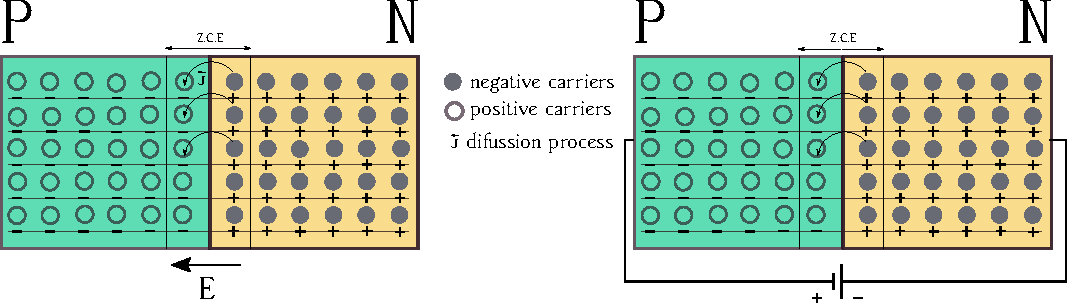
\includegraphics[width=0.6\textwidth]{figs/unionpn.pdf}
% \caption{PN junction, b) PN forward bias}
% \label{fig:pn}
% \end{figure}


% When the equilibrium is reached, the closer region to the interface called \textbf{space charge region}, the minority carriers are recombined and there are only electrically charged ions linked to the net. The electric field created by the ions generates a potential difference called, thermodinamical potential, that avoid the mjoroty carriers to cross to the other side f the juntion.

% \subsection{P-N forward bias}

% If we want to make a current to cross the P-N junction it is necessary to break the balance and that means that you need to reduce the thermodinamical potential. In order to do that, we can apply a potential difference between the edges of each semicunductor. If the P side has a positive voltage with respect to the N side, the PN junction is forward bias and reverse in the other case. In the forward biases the potential barrier is reduced and then electric charge cannot compensate the diffusion. The carriers of each side can go through the charge area and reach the other side, where they are minority carriers. At this moment the diffusion process creates two currents with two opposite directions, so they do not compensate each other and it generates an usable current. 

% If the P-N junction is reverse biases, which means that the P side has a negative voltage, the potential barrier increases and there will not be an usable current.

% Los procesos de generación de corriente en la unión P-N pueden resumirse en la ecuación de Shockley \ref{eq:shockley} que define la corriente generada por un diodo. El diodo es el dispositivo electrónico que se basa en el funcionamiento teórico de la unión P-N. En \ref{eq:shockley} $I_0$ es la corriente de saturación del diodo en oscuridad, $V$ la tensión aplicada y $m$ un factor para ajustar al funcionamiento real y $V_T$ el potencial térmico.

% The processes of current generation in the P-N junction can be summarized in the Shockley equation \ref{eq:shockley} that defines the current generated in a diode, an electronic deviced based in the P-N functioning. In \ref{eq:shockley} $I_0$  is the saturation current, $V$ the voltage applied and $m$ is a factor to adjust to real behaviour and $V_T$ is the thermodinamical potential.


% \begin{equation}
%   I_{D}=I_0\cdot [e^{{V}\over {m\cdot {V_{T}}}}-1]
% \label{eq:shockley}
% \end{equation}

% \subsection{Solar Cell}

% When the P-N junction is iluminated, the incident energy can be absorbed by the electrons in the semiconductor that can jump into the conduction band, due to the photoelectric effect. Charge carriers are produced in this process because a pair electron-hole is created, this pair of carriers is then conducted due to the electric field of the junction creating a current.  

% The equation \ref{eq:Isolar} determine the generated current by an iluminated solar cell.

% \begin{equation}
%   I=I_L - I_0\cdot [e^{{V}\over {m\cdot {V_{T}}}}-1]
% \label{eq:Isolar}
% \end{equation}


% The generated phtotocurrent will depend in the first place on the energy of the incident ligth. If its frequency is not high enough, the ligth will not be able to break bonds and it will go trough the cristal without being absorbed. Due to that not all the ligth can be usable to generate current and it will exist some loses of transmission, reflection and recombination of some of the carriers.

% The equivalent equation of solar cell that makes possible to model its behaviour is based on a current generator and a diode. It can be described by the next equation:

% \begin{equation}
%   I=I_{sc}[1-exp({\frac{V-V_{oc}+I\cdot R_s}{m\cdot V_T}})
% \label{eq:Ieq}
% \end{equation}

% Where $I_{sc}$ is the \textit{short-circuit} current, obtain when the voltage applied to the junction is 0:

% \begin{equation}
%   I_{sc}=I(V=0)=I_L
% \label{eq:Isc}
% \end{equation}

% In addition, if we apply the condition of \textit{open circuit} to the solar cell equation (I=0):

% \begin{equation}
%   V_{oc}=V(I=0)=m\cdot {\frac{k\cdot T_c}{e}}\cdot ln({\frac{I_L}{I_0}}+1)
% \label{eq:Voc}
% \end{equation}

% Finally $R_s$ in \ref{eq:Ieq} represents the resistance due to semiconductor material and the metallic contacs.

\section{Links between climate and renewable energy}

The energy sector and in particular, the electricity power sector is highly dependent on the state of the atmosphere. For the renewable energy technologies, the amount of resource available at each time determine the final energy that can be generated. In addition, the meteorological conditions impact in the electricity demand most notably in extreme events like heatwaves or cold spells.

The energy market and different stakeholders, as well as the need of keep balance between supply and demand, requires an accurate and high resolution meteorological information in order to predict the amount of energy that can be generated with each technology. 

On the other hand, meteorological conditions also affect indirectly in other aspects. For instance, the maintenance and operating activities in an offshore wind farm are a complex process due to the accessibility of the wind turbines. To know beforehand the weather forecast is necessary in order to plan the activities and avoid the risk exposure of the employees.

Although the short-term activities are in the core of the operational side of a renewable energy project, there are also some stages that requires the study of longer temporal scales. Firstly, in order to establish the suitability of a renewable power plant, it is necessary to develop a resource assessment phase or potential assessment phase. This allows the owners to estimate the maximum power output of a project depending on the meteorological conditions and assess the amount of energy that they will be able to produce, what becomes important in order to finance the project.  

The term bankability makes reference to the suitability if a project of being profitable and reliable to financing. In order to determine that, long term information about the resource is considered in renewable projects. Bankabilkity [ref] of a project depends on two main factors: in first place the availability of the resource and in the second place the benefits obtained from the project. Benefits depends on the operation time and the amount of energy supplied during the lifetime of the project. Due to that, an accurate assessment, not only of the available resource, but also of its variability and trends, is necessary. 

The relevance of the seasonal and sub-seasonal scale for the operation and maintenance of power plants has to be noticed. The improvement in the climate forecast on that scales will impact directly on their activities and will help to the TSO and market operator in the management activities. For instance, to know in advance if the next Autumn is going to be specially rainy, will help to assess the amount of electricity the can be produced with hydro-power plants, making the system more reliable and efficient.

\subsection{Climate change and the energy sector}

In a global warming context, the link between energy and climate has been usually related to the impact that a big share of renewable in the generation mix can cause regarding the possible reduction of GHG in this way. However, the fact that climate change can cause at the same time variations in the availability or distribution of the resources, as well as in the electricity demand patterns, should be taken into account and thoroughly researched. 

One of the associated problems to the possible medium to long-term changes on the renewable resources, like the wind patterns, is the possibility of profitability loss of some projects that are now in the final stage of their lifetime. Repowering of these projects with upgraded technology, like the replace of old wind turbines by new ones with larger nameplate capacity or more efficient, is one of the options for the power plants installed almost two decades ago \cite*{delrio}. Changes in the resource can change the conditions of the project because of the turbines used and because of the availability of the resource.  


%{\color{red} AQUÍ PUEDO HABLAR DEL IMPACTO EN NUCLEARES, TÉRMICAS, CABLES ETC}

In addition, the rising temperature due to climate change can directly affect the energy generation and infrastructure in different ways. For the conventional power plants, that increase in air temperature means a decrease in their conversion efficiency as well some problems related to their refrigerating activities.

The projected increase in extreme events also have potential hazards and risks for the industry that have to be considered. One example is the increase in the temperature of the river flow due to the above normal air temperature in a heatwave episode, which are projected to be more frequent and severe [ref]. That increase can affect the nuclear power plants operations, because the impacted plants are not able to use the river for their refrigeration purposes [ref]. Also, the more frequent drought events impacts directly hydropower generation.  

The energy infrastructure can be also be affected by the increasing temperature. The exposure of air transmission lines to higher temperatures impacts its capacity. In addition, under extreme events they can be damage in rainfall episodes or extreme winds. 
%{\color{red}It is relevant to say that conventional power plants can get profit of the climate services information. Some of them can easily be impacted by some extreme events like heatwaves. The above normal air temperature in a heatwave episode can be related to the increase in the temperature of the river flow. That increase can affect the nuclear power plants operations, because the impacted plants are not able to use the river for their refrigeration purposes [ref].}   


\begin{figure}[h!]
\centering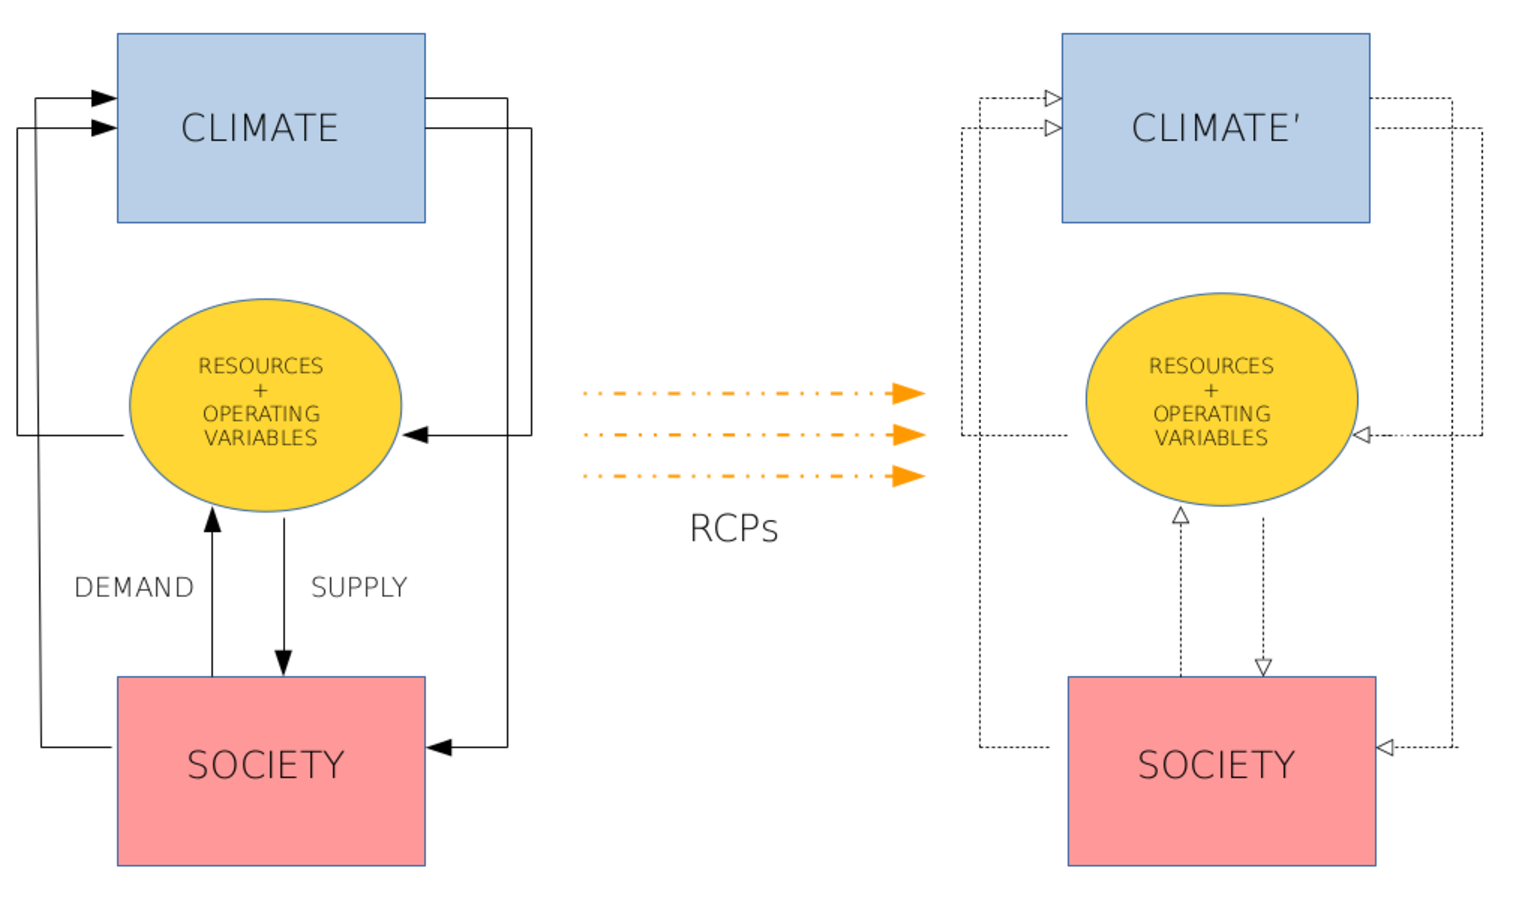
\includegraphics[width=0.6\textwidth]{figs/esquema.pdf}
\caption{Scheme: conceptual representation of the relationships between climate, energy sector and societies. Left side of the scheme represents actual conditions and right side is the future relationships after the evolution following an RCP scenario. }
\label{fig:feedback}
\end{figure}

 
%La bancabilidad[ref] de un proyecto renovable depende de dos factores: en primer lugar su recurso y en segundo lugar, sus beneficios. Los beneficios obtenidos por el proyecto renovable dependerán del periodo de operación y de la cantidad de energía suministrada en este tiempo. Por ello, una evaluación adecuada, no sólo del recurso disponible a lo largo de todo el proyecto, sino de su variabilidad y de las posibles tendencias, es necesario a lo largo del ciclo de vida de la planta, que puede alargarse hasta 30 años[ref].



%En la figura... están representados diversos eventos meteorológicos y climatológicos que afectan a la generación energética. El eje 'x' representa las distintas escalas temporales en las que ocurren estos eventos. Es interesante destacar, aunque no es el tema principal de esta investigación, la relevancia de la escala estacional y sub-estacional para la operación de las plantas energéticas de tipo renovable. La mejora en la predicción climática en estas escalas repercutirá de forma directa en la planificación de la operación y mantenimiento, así como ayuda en la gestión por parte del operador de red y mercado. Por ejemplo, conocer con antelación si un otoño va a ser especialmente lluvioso, sirve para predecir la cantidad de electricidad que se puede producir con las centrales hidroeléctricas, haciendo el sistema mucho más eficiente y fiable. 



% !! escalas climáticas: ¿es importante la repotenciacion? tener en cuenta esto? mismo recurso en el futuro?
% !! infraestructuras y extremos climáticos.


\subsection{Climate services}

%Con la creciente demanda de información por parte del sector energético de predicciones y proyecciones climáticas, aparece de manera natural la creación de los servicios climáticos para sistematizar, de alguna manera la información necesaria para los distintos stakeholders. 

Due to the intrinsic characteristics of renewable energy resources, related to their high space-time variability and the potential impacts on the energy sector mentioned above, there is an increasing demand of information about many climate forecast, projections and hazards. Although the energy sector is one of the most interested in the development of an operational system of climate information, there are also other sectors that would benefit from that, like agriculture or tourism.  
  
This increasing demand of predictions and climate projections from different sectors, has lead to the development of the  climate services, in order to systematize, to org anise and to target the information for different stakeholders. [ref]

%Como puede observarse en la figure \ref{fig:feedback}, los procesos de interacción entre la sociedad y las variables involucradas en la generación de energía son de doble sentido. Por un lado el abastecimiento dependerá de la disponibilidad de los recursos y por otro, la demanda está directamente influenciada por estos factores climáticos. Teniendo en cuenta esto, el desarrollo de los servicios climáticos debe basar la mejora de sus modelos y por lo tanto, de los productos ofrecidos en estas dos premisas.

From the renewable energies side, climate information is specially relevant for strategic decisions, evaluation risks, planning and trading operations. As can be seen in figure \ref{fig:feedback}, interaction processes between society and the variables involved in the energy generation are two-way relations. On one hand, the energy supply would depend on the availability of the resources and constrains due to climate change;  and on the other hand, demand is directly influenced by those factors. Due to that, development of climate services should be based on the improvement of the models and the offered products considering the two sides.   

%La información climática en el sector energético es especialmente relevante para las descisiones estratégicas y la evaluación de riego, las operaciones de trading o la planficación de la operación y el mantenimiento en las plantas de generación (especialmente) renovables.



%Es relevante, aunque no es el tema de esta tesis, decir que también otros tipos de generación no renovable pueden beneficiarse de esta información y estar afectados de manera importante por algunos eventos climáticos. Por ejemplo, el aumento de temperatura del aire puede provocar una subida en la temperatura de los ríos, que ocasionalmente repercute en la operación de las plantas nucleares. En estos casos, estas plantas se ven afectadas porque no pueden continuar on las operaciones de refrigeración de los reactores (ref). 


%\section{Resource assessment}
\section{Climate change and the Mediterranean area}

% \begin{itemize}
% \item Cambio climático de origen antropogénico a escala global. Aumento de la temperatura global.
% \item Los impactos del cambio climático ocurren en escalas locales o afectan de manera local a distintas comunidades y poblaciones de una forma desigual, relacionada también con su capacidad de adaptación y resiliencia.
% \item Por las razones mencionadas arriba, la respuesta a los diferentes impactos de cambio climático deben adoptarse de manera local, a pesar de que el consenso sobre la urgencia de actuación sea global y se adopten compromisos globales comunes.
% \item La mitigación de los grandes impactos ocurre en escala regional/local.
% \end{itemize}

%El sistema climático ha variado continuamente y de manera significativa a lo largo de la historia de la Tierra. Las variaciones del clima puede explicarse debido a factores o forzamientos externos y la respuesta del sistema climático a los mismos o, por otro lado, puede ser la causa de inestabilidades internas y relaciones no lineales entre los distintos componentes del sistema.

Climate system has varied constantly and significantly along the Earth's history. Climate variability can be explained due to external factors and the response of climate system to them or, on the other hand, due to the internal instabilities and non-linear relationship between different components of the system, occurring the last ones with independence of the external forcings.

%Los distintos forzamientos de origen externo pueden ser factores astronómicos, como los cambios en la intensidad de la radiación solar o en los parámetros orbitales, o bien, factores terrestres como la composición de la atmósfera debido a la actividad humana, cambios en la superficie terrestre debido al uso de la misma etc.

External forcings can be astronomic factors, like changes on the intensity of solar radiation or in the orbital parameters, or they can be terrestrial factors like changes in the composition of the atmosphere due to human activity, changes in the earth's surface due to land use etc.

%Algunas variaciones del sistema climático ocurren de manera independiente de los forzamientos externos. Estas variaciones tienen su origen en las distintas interacciones no lineales entre los componentes del sistema climático y dan como resultado la variabilidad natural del sistema climático. 

%Some variations of the climate system happen independently of the external forcings. These variations have their origin on different no-linear interactions between different components of climate system and the result is the natural variability of the climate system.

%Desde la revolución industrial la Tierra ha experimentado un aumento de la temperatura global que no es posible explicar mediante los forzamientos externos 'naturales'  del clima como cambios en la actividad solar o en las emisiones volcánicas (Bindoff et al, 2013), ni forma parte de la variabilidad natural del sistema. El IPCC en su último informe, asegura que la actividad humana y en concreto las emisiones de efecto invernadero generadas desde la Revolución Industrial (1850) son responsables del cambio climático que ha generado el ascenso de temperatura global y que ha hecho que probablemente los 30 años entre 1983-2012 hayan sido los más cálidos en los últimos 1400 años en el hemisferio norte (IPCC). A pesar de la marcada variabilidad interanual (Stocker et al. 2013), el aumento de temperatura con caracter global en las últimas décadas es evidente. [ref de observaciones globales]

Since the Industrial Revolution the Earth has experimented an increase in the global temperature that cannot be explained due to natural external forcings like changes on solar activity or volcanic emissions (Bindoff et al, 2013), either it cannot be explained as part of the internal variability of the system. The IPCC in its last report, assure that human activity and more precisely, GHG emissions generated since 1850 are responsible of the climate change that causes the increase in global temperature and has made that probably the last 30 years between 1983-2012 have been the warmer in the last 1400 years in the northern hemisphere (IPCC). In spite of the large interannual variability (Stocker et al 2013), the global character of the temperature increase in last decades is clear.[ref de observaciones globales].

%Las consecuencias del aumento de temperatura desde un punto de vista físico dependen de la sensibilidad del sistema a los cambios en la concentración de gases de efecto invernadero. Son numerosos los estudios [ref] que se han realizado para intentar cuantificar el impacto que este aumento de temperatura puede tener en los distintos subsistemas a través de los diferentes mecanísmos de retroalimentación que pueden generarse.

%A pesar de la característica global del cambio climático, sus consecuencias e impactos son percibidos a escala local y regional. Estos impactos afectan a comunidades y poblaciones de manera desigual dependiendo de su capacidad de adaptación y resilencia. Por ello, la respuesta desde un punto de vista socio-económico para mitigar estos efectos, tiene que venir dada en esta escala, aunque exista consenso sobre la urgencia de actuación y se adopten compromisos comunes.

Despite that climate change is a global concept, its consequences and impacts are perceived in a local and regional scale. These hazards and impacts affect communities and population unequally depending on its vulnerability, adaptation capabilities and resilience. Due to that, the socio-economic response to mitigate climate change impacts has to be applied in that scale although it should be a consensus on the urgency and some common compromises have to be adopted.

%Uno de los primeros trabajos que intentaba cuantificar el impacto del cambio climático a escala local fue el de Giorgi et. al 2006. En este trabajo, se utilizaba por primera vez un índice (RCCI) para medir de forma cuantitativa y compara geográficamente las zonas más afectadas por el CC. En este aspecto, el trabajo estaba enfocado desde un punto de vista climático, es decir, el índice mide la sensibilidad del clima en esa zona. En este sentido, el Mediterráneo aparecía como una de las zonas más afectadas y desde entonces ha sido denominado como un hot-spot de CC.

One of the first works on quantification of climate change impacts in a regional scale was the one published by Giorgi in 2006 \cite*{Giorgi2006}. They used for the first time an index, RCCI, to measure and compare geographically the climate sensitivity of different areas to climate change. The conclusion of the research showed the Mediterranean area as on of the most affected area in terms of climate response to climate change, and since then it has been refereed to as a climate change hot-spot.

%Los ensembles de modelos climáticos proyectan escenarios en los que las principales consecuencias del calentamiento global en el área Mediterránea son un descenso generalizado de las precipitaciones, debido a un aumento de la circulación anticiclónica asociada a un desplazamiento hacia el norte de ``Atlantic storm track''. Las temperaturas proyectadas son inusualmente altas con un ascenso especialmente alto en los meses de verano.

The climate models projects scenarios in which the main consequences of global warming in the Mediterranean area are a generalized decrease of precipitations (with the exception of some areas like the Alps), due to an increase in the anticyclonic circulation, that is associated with a northward shift of the Atlantic storm track [ref]. Also it is projected an increase in interannual variability of temperature and precipitation, mostly in the warm season \cite*{Giorgi2008}. In terms of extreme events, it is also projected less frequent but more intense precipitation events and with respect of temperature, some authors have evaluated the probability of an increase in heatwaves over the Mediterranean area [ref]. All this climate perspectives and consequencies of the global warming,  should be considered in order to plan and prepare the adaptive capacity of the region.\\   

\section{Organization of the manuscript}%\section{General scientific question: spatiotemporal variability of solar resource and photovoltaic production}

This manuscript is organized as follows:

The \textbf{first part} of the text contains two chapters: the first one is the previous \textbf{Introduction}, that aims to introduce the context in which the thesis has been elaborated. In the second chapter, \textbf{State of knowledge}, there is an introduction on the main contributions related to this topic over the literature. It includes a general overview about intermittency of PV and how the short-term problems has been managed. After that, the long-term problems and the main contributions about this topic over the area are reviewed. %Also, the climate change perspective over the Mediterranean region and the main literature related to solar resource is revised.

The \textbf{second part} is composed by two chapters including the \textbf{Data} description and the \textbf{Methodology} used along the studies. In this case it is important to remark that each results chapter has its own 'Data and Methodology' section used for that specific chapter. The contents of this part II are related to general description of ground stations, satellite, climate data and models as well as general methodologies.

The \textbf{results} are presented in the \textbf{third part} of this manuscript. There is a different chapter for one of the main aspects investigated here and described in the above section. The organization of this chapter is being adapted from the journal papers where these results have been published.

Finally the \textbf{fourth part} contains a chapter with some \textbf{discussion} and limitations about the results previously presented and the main \textbf{conclusions}. This section also summarizes the main questions emerged from the work, which will lead future research.

% \section{State of the art}
% \subsection{From short to long term varibility issues}
% \subsection{Solar radiation data measurements}
% \subsection{Satellite data}
% \subsection{Modelization of solar radiation}
% \section{Identification of knowdlege gaps and approach to the problem}
%\subsection{Spatiotemporal long-term variability in an almost isolated area}
%\subsection{Role of aerosols in the spatiotemporal varibility of the photovoltaic energy production}
%\subsection{Future availability of photovoltaic potential}

 
\chapter{State of knowledge\label{cha:state}}

% \epigraphfontsize{\small\itshape}
% \epigraph{''Commençons par les systèmes les plus simples et les plus faciles à cerner pour monter graduellement à la compréhension des plus complexes.''}{--- \textup{René Descartes}, Le Discours de la Méthode}

\section{Variable renewable energies: VRE}

The variable nature of renewable energy resources, in space and time, is a key aspect for their high penetration into the conventionally designed electricity systems. Due to the requirement that supply and demand have to match at every time-step, the forecast and management of the generated electricity is needed for accomplishing this match, which becomes more difficult in the case of variable renewable energy (VRE) plants.

In the traditional electricity systems, a portfolio of centralized power plants (coal, nuclear, gas...) dispatches electricity as the customer loads demand it. The conventional power plants are able to storage the primary energy that they use and produce electricity only when it is needed. With the increase of renewable power plants, mostly wind and solar, the supply of electricity demand approach has changed. The VRE power plants only produce electricity when enough resource is available and in the case of photovoltaic power plants, only during the daylight time. This concept has being referred as \textbf{intermittency}, to recall the fact that solar and wind resources are not available at any time and that they are variable by nature. Nevertheless, there are renewable power plants that are able to provide energy by demand, like biomass power plants or hydropower (with some restrictions in drought events). They are dispachable and can operate as the conventional thermal power plants.

Due to the rising penetration of the non-dispachable power plants (wind and solar) the management  and the operation of the system has to be adapted. However, the alternatives for energy storage for VRE plants are increasing in different ways: batteries for wind and photovoltaic power plants, hydrogen or pumping hydro-power \cite*{Lund2015, Blanco2018, Schaber2004}, which favors the integration of the alternative energy sources.

The research in storage for VRE is rising but different approaches are also being adopted to integrate high share of this alternative technologies. The term \textbf{flexibility} is one of the most used referred to the new strategies followed from the demand and supply side in order to adapt to the new system \cite*{KROPOSKI2017}. From the demand side, flexibility refers to means related to load shape and demand patterns, like peak saving, load shifting, valley filling etc \cite*{Lund2015}.

On the other hand, flexibility of the supply side depends on the power plants, whose output can be controled to obtain power balance. It is important in terms of flexibility to consider the response time of different power plants as well as the different nature of each one. As the availability of solar and wind resources are not related to the geographical distribution of the demand, a highly interconnected grid is one of the main needs for a high penetration of VRE. Once this is considered, geographically spread portfolio of VRE plants are able to smooth variability of power output \cite*{KROPOSKI2017, Marcos2012}(Hoff and Perez 2012, 2013, añadir más referencias).

%* Explicar más el concepto de smoothing?? agregar aquí todas las citas de smoothing

There are also studies that try to identify complementary features of different energy resources, either in time or in space, in order to address the intermittency issue through the smooth of the total power output. The complementary studies are made using different technologies like hydro-power and wind power \cite*{Denault2009, Silva2016} or hydro-power and solar photovoltaic \cite*{Francois2016, Beluco2012, Kougias2016}. In \cite*{Hoicka2011} complementary of wind and solar is investigated for a region in Canada and also in Italy \cite*{Monforti2014}.  In addition, over the Iberian Peninsula \cite*{Santos-Alamillos2012, Jerez2013b} and Great Britain \cite*{Bett2016} it has also being investigated from a more climatological approach.

As much as we were able to forecast the variability of solar/wind resources in the short term and in to characterize the resource in the long-term to  estimates and project the energy to be produced, better flexibility measures and strategies could be apply to integrate high rates of VRE without compromise reliable and efficiency.

% For example on the supply side, the kind of flexibility is accomplished through power plants with
% different response time. Introducing variable power generation such as wind and solar power may
% increase the need of energy system flexibility, which could be accomplished through additional measures
% on the supply or/and demand side which is the subject of this paper. From the electricity system point of
% view, flexibility relates closely to grid frequency and voltage control, delivery uncertainty and variability
% and power ramping rates
\section{Variability sources in PV}

It is important to notice that every power system has associated an inherent variability and uncertainty, as a non-exclusive characteristic of a renewable energy system. In the case of PV systems, the variability of PV outputs depends on two items: on the first place, it depends on the variability linked to the solar irradiation reaching the generator (resource variability), and secondly, it also depends on the behavior of the electrical components.   

% ``Before focusing on the variability and uncertainty of PV plants, it is important to understand that
% variability and uncertainty are inherent characteristics of power systems. Loads, power lines,
% and generator availability and performance all have a degree of variability and uncertainty
% It is clear that uncertainty in photovoltaic power it is a combination of the uncertainty of estimation of solar resource and the uncertainty in the behaviour of the electrical componentes of the photovoltaic system.''
Solar radiation varies in multiple time-scales, from seconds to multi-decadal variations, as well as spatially, affecting PV production. For the operating activities in PV plants, an accurate forecasting of solar irradiation, which means, being able to reproduce its short-term variability, leads to better forecasting of the PV output, demanded by TSOs and used for trading. In longer time-scales, to understand variability features improves the projection of the PV output for a period of time: seasonal, year-to-year produced energy, multi-year trends or climate change projections. That helps in the plannification, the strategy, the financing activities, and can influence in the policymakers decisions.

Different factors are responsible of the variability either of solar resource or the electrical components of the PV generator and affect them across different time and spatial scales.

\subsection{Astronomical factors}

The amount of solar energy that reaches the photovoltaic generator depends on the first place on the sun position with respect to the orientation of the PV panels, which is a deterministic factor that only depends on the time of the year, the time of the day and the relative position of the generator surface. It means that the first factor causing PV intermittency is the fact that no energy can be produced during night-time. However, although this daily scale intermittency is the one that most affects the PV power production there is no uncertainty associated to this fact, which is a very important concept in order to manage VRE.

\subsection{Atmospheric factors}

\subsubsection{Clouds}

There are other factors that reduce the amount of solar energy reaching the surface and their influence depend on the composition of the atmosphere at each time. When solar radiation goes through the atmosphere it can be reflected, absorbed or scattered. The presence of clouds is the most affecting factor in the transmission of solar radiation to the surface. The condensed particles that forms clouds makes solar radiation being scattered and reflected and part of the radiation can also be absorbed. Different types of clouds affects differently to solar radiation \cite*{Page2012}. High thin clouds are less dense than low clouds, becoming more transparent to solar radiation \cite*{Kasten1980}. %Also, some clouds are less spatially aggregated than others. When the sky is overcasted, the amount of energy reaching the surface decrease but the frequency of the intermittency generated in the PV output is not as high as if some individual clouds pass through.

For partially cloudy skies, solar irradiance (direct component) can drop in seconds \cite*{Page2012} due to clouds. In overcasted periods, short-term variations depends on the type of clouds.

Low frequency changes in cloud cover for large areas are related to changes in large scale circulation patterns, which is linked to changes in solar resource for that places \cite*{Chiacchio2010, Sanchez-Lorenzo2009}.

%{\color{blue} Incluir referencia del libro: practical handbook of photovoltaics funcdamentals and applications para tipos de nubes y su transmitancia y otras referencias}
\subsubsection{Aerosols}

Aerosols is the term used to referred to the solid particles suspended on gas. In this work we are referring to the atmospheric aerosols, which are the solid particles suspended on the atmosphere but the hydrometheors like ice crystals \cite*{boucher2015}. In the absence of clouds, aerosols are the main source of variability for solar resource. 

Aerosols impact solar radiation in two ways: directly, scattering, absorbing or reflecting solar radiation or indirectly, acting as condensation nuclei favoring the formation of clouds \cite*{boucher2015}. They can be classified depending on its source origin. Natural sources emit aerosols from oceans, wild fires and vegetation, whereas antrophogenic sources emit aerosols from industrial activities, burning fuels and human-caused fires.

%  Natural sources consist of emissions from
% the ocean, soils, vegetation, fires, and volcanoes. Anthropogenic sources are
% largely dominated by emissions from the combustion of fossil fuels (i.e. coal
% and oil), biofuels (plant biomass including wood, vegetable oils, animal waste),
% other fuels (e.g. peat), or vegetation fires caused by humans. Industrial activities,
% transportation, heating, or even domestic activities related to cooking in developing
% countries, are important sources of aerosol

Aerosols vary greatly in time and across space \cite*{Kaufman2002}. Besides of aerosols relatively short residence time in the atmosphere (of the order of hours to weeks), they have an strong influence on climate through their impact on the radiative budget and clouds \cite*{Nabat2015, Nabat2015a}. Aerosols from natural sources, like mineral dust airbons, which last some days, have a very strong seasonality, affecting in regional and continental scales periodically.  Also, due to the relationship between aerosols and human activities, long time cooling trends have been detected in China for last decades related to the increase in aerosols optical thickness (Giorgi 2002) and other studies had shown the relationships between the ``dimming'' and ``brightening'' and the antrophogenic aerosols emissions \cite*{Wild2005, Wild2012, Wild2009}. 

%{\color{blue} Falta incluir referencias: A satellite view of aerosols in the climate system Kauffman 2002}
%Gueymard, C.A. Temporal variability in direct and global irradiance at various time scales as affected by
%aerosols. Solar Energy 2012, 86, 3544 – 3553.

\subsection{PV system factors}

\subsubsection{Spatial aggregation}

There are two factors related to the spatial dimension that influence on the photovoltaic power variability:

\begin{itemize}
\item {Power plant size}
  A PV power plant acts like a low-pass filter for short-fluctuations, which means that higher frequencies of power fluctuations (less than a minute) from the PV generator are smoothed as a function of the PV plant size \cite*{Perpinan2011, Perpinan2013}.
\item {Distance between power plants}
  On the other hand, it has been also concluded that for a fleet of dispersed PV plants, short-term power output fluctuations are attenuated. Some authors observed that short-term fluctuations are essentially uncorrelated for distances between PV plants over 6 km.\cite*{Otani1997, Wiemken2001, Hoff2012}
\end{itemize}

%{\color{red}Another important factor that affects PV output fed into the grid is the PV generator size or even distance between different PV power plants. In the short and very short time scales,  This is called te smoothing effect and it can be used as one of the strategies to follow in order to address the variability issue of renewables.}

\subsubsection{Other factors}

As it has been noted at the beginning of the section, there are other factors that affects the performance of a PV system, causing variations in the power output. These factors are related to the electrical components of the system and they can be divided into internal and external factors.

The most important external factor affecting the PV system is temperature. It affects cells performance and if temperature is highly different than the optimum cell temperature the efficiency will drop. Also some external factors like dust deposition can affect the electrical performance, limiting the energy reaching the cell \cite*{Fan1986, Mekhilef2012,Dubey2013}.

Internal factors affecting the PV output that can cause variability are related to the transmission lines, wires and interconnections, or the inverter, whose functioning is not always constant and can present variations.

\section{Short-term variability}%Photovolatic power forecasting

%Considerando los distintos factores que intervienen en la variabilidad de la producción fortovoltaica antes mencionados, queda reflejado que el estudio de la variabilidad puede hacerse bien desde el punto de vista del recurso, es decir, de la radiación solar en superficie o incidente en el generador, o bien desde el punto de vista de la generación eléctrica.[widen]

From the different factors that influence in variability of PV power production, it can be followed that variability studies can be made through the solar \textbf{resource} point of view or from the \textbf{power} variability side \cite*{Widen2015}.
%El estudio de la variabilidad a corto plazo desde el punto de vista del recurso ha venido ligado a la ivestigación sobre la caracterización del la radiación solar en superficie. Algunos de estos estudios tenían como objetivo únicamente el modelado estadístico del comportamiento de la radición en escalas temporales cortas [Liu] y otros estaban motivados por el desarrollo de la energía solar fotovoltaica y la necesidad de caracterizar el recurso para el mejor funcionamiento de las mismas.[collares pereira] 
%{\color{blue} HAY QUE METER VARIABILIDAD POR AEROSOLES}

\subsection{Resource Variability}

% El estudio de la variabilidad a corto plazo desde el punto de vista del recurso ha venido ligado a la ivestigación sobre la caracterización del la radiación solar en superficie. Algunos de estos estudios tenían como objetivo el modelado estadístico del comportamiento de la radiación en superficie en escalas temporales cortas [Liu] y otros estaban motivados por el desarrollo de la energía solar fotovoltaica y la necesidad de caracterizar el recurso para el mejor funcionamiento de las mismas.[collares pereira] En este sentido, el estudio de variabilidad ha sido generalmente de carácter local.

The research of short-term variability from the resource perspective, has followed the research about the characterization of solar irradiation at the surface. Those studies had the objective of the statistical modeling of solar irradiation behavior at the Earth's surface in short-term time scales \cite*{Liu1960}. Others, were motivated by the solar energy development and the need of characterize the resource for a better performance of the PV plants \cite*{Collares-Pereira1979}. In that sense, variability studies has been generally focused with a local character.

%{\color{red}Para las distintas operaciones en el corto plazo, predecir la cantidad de energía que un generador o planta fotovoltaica va a verter a red, ayuda a a la gestión de la intermitencia inherente a la producción fotovoltaica. Para ello, será necesario en primer lugar predecir la energía solar incidente en el generador fotovoltaico y en segundo lugar modelar el comportamiento del generador fotovoltaico para predecir la AC producida.}

For different operation activities, to forecast the amount of energy fed into the grid from a PV system or plant, is essential in order to manage the associated intermittency to the photovoltaic power production. In order to accomplish that, it is needed on the first place to forecast the amount of incident solar energy on the photovoltaic generator and secondly, to model the system's behavior in order to forecast the AC produced.   

%lleva a analizar PV production 'ramps' provocadas por cambios en la radiación solar incidente asociados al movimiento de nubes y el efecto 'smoothing' antes mencionado. En este aspecto, la escala temporal está relacionada con el grado de 'suavidad' que se puede alcanzar con la agregación espacial de distintas plantas fotovoltaicas.

% Por otro lado, el tamaño del generador es un factor que ha sido estudiado para determinar la variabilidad en escalas de tiempo entre tal y tal, observándose que :

% he main research question in current solar variability research is which degree of smoothing of the intra-hourly fluctuations can be achieved with different degrees of geographical dispersion of irradiance sensors or PV systems (see Section 4.4). Current research efforts are in particular focused on determining the relationships between cloud speeds, correlations between sites, time resolution and overall variability. Previous overviews of the field can be found e.g. in [1,8,70,71]. The time scales focused on in current research on solar variability range from several minutes down to seconds. The
% relevant time scale depends on the correlation between these sites, which in turn depends on the distances between them. The shorter the time scale, the faster the decline in correlation. Determining the variability for completely correlated or uncorrelated ensembles of systems is straightforward [72], while the range in-between is non-trivial. For example, [70,73,74] and other studies indicate that close-to-zero correlation is reached at a few up to tens of km for resolutions of seconds or minutes, which is the spatial and temporal scale least explored in existing research
% [70,75].

% Also, the smoothing effect that a well-spread site planning has on the PV production is being investigated: [Mar+12], [PML13].

 
%{\color{red} Como se ha comentado anteriormente, para las distintas operaciones en el corto plazo, predecir la cantidad de energía que un generador o planta fotovoltaica va a verter a red, ayuda a a la gestión de la intermitencia inherente a la producción fotovoltaica. Para ello, será necesatio en primer lugar predecir la energía solar incidente en el generador fotovoltaico y en segundo lugar modelar el comportamiento del generador fotovoltaico para predecir la AC producida.}
  
%The energy that is obtained from a photovoltaic system can be forecasted in advance if the amount of solar energy that reach the generator surface is accurately predicted. The prediction of solar irradiation variability enhance the forecast of the energy output. After that, it is necessary to model the electical components of PV generator. 

%%%%%%%%%%%% ELimino esto porque es un lío con lo de clear sky pero tengo que coger alguna referencia (Tovar)%%%%
%There are different types of forecasting methods for solar power, they are based on the models that forecast solar irradiation. Among them there are two different approaches: \textbf{physical methods} and \textbf{statistical methods}. Physical methods are based on the radiative transfer equation and physic variables whereas the statistical or empirical methods are based on historical data. Some approaches are also \textbf{hybrid} approaches that combined both \cite*{Diagne2013, Tovar-Pescador2008}. They mainly rely on two principles: first an estimation of the clear-sky irradiance and secondly, they account for the presence of clouds [ref Jan Kleiss].  


\subsubsection{Solar irradiation forecasting}

There are different types of forecasting methods for solar irradiation. There are two different approaches: \textbf{physical methods} and \textbf{statistical methods}. Physical methods are based on the radiative transfer equation and physic variables whereas the statistical or empirical methods are based on historical data.

The application of each kind of the forecasting models is very related to the \textbf{forecast horizon} that want to be addressed, as well as the horizontal resolution. In the operation activities, 3 time forecasting horizons were described by Kostylev and Palovsky \cite*{kostylev2011solar}: intra-hour, intra-day, day-ahead. For other activities like trading, the day-ahead forecast is very important as well as for planning operations. The statistical approach is applied in shorter scales whereas the physical approach has been proved to have a better performance \cite*{Perez2010, Diagne2013, Widen2015}.% in longer time-scales seasonal forecast will be a very valuable asset if model skill improves [ref]. 

\begin{itemize}
\item{Physical Methods}

The physical modeling of solar radiation is based on physical equations of the interaction between atmospheric components and solar radiation (aerosols, water vapor, clouds...). When solar radiation goes through the atmosphere, it can interact with its components being absorbed by molecules, back-scattered to space or scattered in any other direction. Thus, only part of the solar radiation at the top of the atmosphere (TOA) will reach the Earth's surface.

This process is the physical process of energy transfer described by the radiative transfer equation (RTE) and its solution needs a radiative transfer model (RTM). The radiative transfer is a very complex process that needs to be simplified to be solved numerically and some parametrizations are needed. However, from these models it is possible to reproduce the solar radiation behavior across the atmosphere and at the surface. RTMs are in the core of numerical weather prediction models, NWP, and climate models and sometimes they are used to obtain solar radiation from satellite images, although in this case empirical or semi-empirical approaches are also commonly applied.

Numerical weather prediction models are very useful in a time range from 4h to 6h and they are also applied for the day-ahead forecast \cite*{Perez2010}. It is very frequent to apply a post-processing process to the output of NWP that enhance the forecast. Some statistical tools like bias correction can be apply to reduce some systematic errors or local effects \cite*{Diagne2013}.

%{\color{red} Introducir aquí que en el desarrollo de NWP no se han incluido aerosoles ?}

\item{Statistical methods}

Solar radiation at the surface can be estimated also using statistical methods. In this case it is necessary to have enough accurate historical data to create and validate the model and likely these models will not be able to reproduce solar behavior universally. However, they can be very useful for local applications and at very high time-resolution.

Under these methods traditionally used to forecast time-series, relies the idea of predict some variables through the statistical analysis of historical data and its relationship with other variables called predictors. Many models have been developed in this sense from the most simple approach, the persistence model or autorregressive models, to more sophisticated ones \cite*{Reikard2009, bacher2009, Inman2013}. Also, with the develop of the ANN, non-linear models have been also applied to solar the forecasting field, with the predictions based on an algorithm learning \cite{Mellit2008}. 
 
%{\color{red} escalas temporales: short term and very short-term. Se analiza el impacto de las nubes -> muy común aplicar un modelo de cielo claro y después la influencia de las nubes. Describir aquí lo que son los modelos de cielo claro?}

%{\color{blue} meter aquí clear-sky models? y que pasa con los de satélite}


% Statistical methods have been used successfully in time series forecasting for
% several decades. Using the statistical approach, relations between predictors,
% variables used as an input to the statistical model, and the variable to be predicted,
% are derived from statistical analysis. Several studies with respect to
% direct time series modeling have been performed. In Reikard [2], different time
% series models are compared. In Bacher and al.[7], the authors investigate the
% use of a simpler AR model to directly predict PV power in comparison with
% other models.

\item{Hybrid methods}

It is very common to apply a combination of more than one model to enhance the prediction accuracy. Many studies have shown the overcome of a combination of two different approaches with respect to a simpler approach \cite*{Diagne2017, Yang2014}. For instance, some studies show the application of ANN methods after the obtention of NWP output \cite*{Cornaro2015} or after obtain a satellite-based model output \cite*{Marquez2013} 

\begin{figure}[h!]
\centering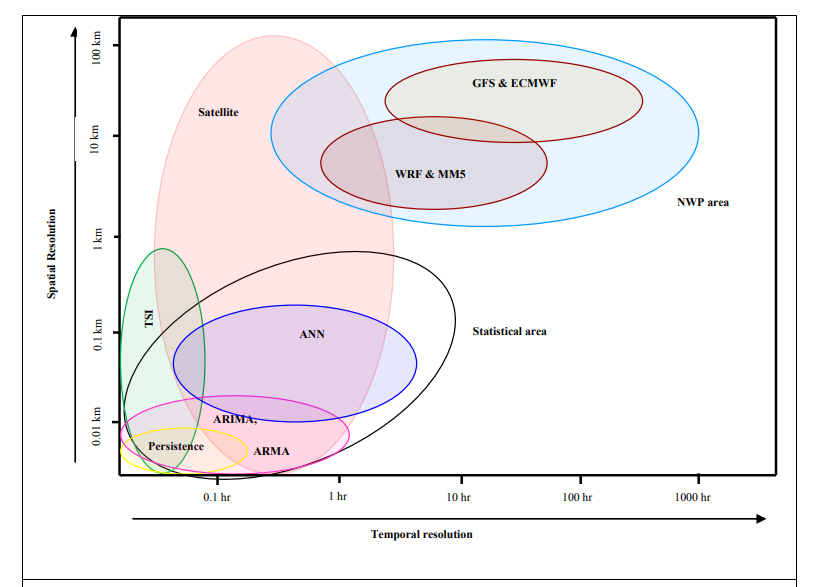
\includegraphics[width=0.6\textwidth]{figs/forecast.png}
\caption{Models to forecast irradiance depending on the time horizon. Incluir ref aunque se va a rehacer}
\label{fig:forecast}
\end{figure}


Different models are applied depending on the forecast horizon as they are summarized in the figure. For shorter periods, statistical methods are preferred to derive solar irradiation from satellite measurements. As far as the time horizon increases, the NWP are used to forecast irradiance.

%Usually, the main steps in the solar irradiation forecast are first the estimation of the clear-sky irradiance and after that account for the presence of clouds ref[Jan Kleiss].

\end{itemize}

\subsubsection{Aerosols in solar irradiation forecasting}

Although clouds are the main driver of variability of solar resource, under cloudless conditions, aerosols reduce the amount of solar energy reaching the earth's surface. Some models compute solar irradiance in clear sky conditions, which means that the they calculate attenuation of solar irradiation only due to the constituents of the atmosphere. Many clear-sky models has been proposed on the literature \cite*{Gueymard2012}. The difference between clear-sky models is based on the parameters used to predict solar irradiance. The most simplest ones only consider the zenith angle and extraterrestrial irradiation. The higher the complexity of the model, the more parameters are included to characterize the state of the atmosphere: different aerosols content, water vapor etc. Performance of this models depends on the parametrizations of each model and the knowledge of the atmospheric composition.
 
These models are commonly used in to derive solar irradiation from satellite observations (see chapter data). As satellite are able to give observations of the cloudiness at a given time and site, the use of a clear sky model in combination with this observation make easy to establish a relationship between the cloud index and the clear sky index . The role of aerosols input in these satellite-based methods to derived solar irradiation has been investigated in \cite*{Polo2014}. 

On the other side, under high loads of AOD, NWP usually presents a systematic bias in solar radiation forecast \cite*{Rieger2017}. This fact is due to the design of the models that normally use climatological values for the representation of aerosols with homogeneous spatially and temporally concentrations. This fact lead to an overestimation of solar irradiation in the dust outbreak of 4 April 2014 in Germany, which caused significant economic losses \cite{Rieger2017}.

%{\color{blue} Aquí podemos hablar de los aerosoles, que impactan en la predicción de la irradiancia porque afectan a su variabilidad. Númerosos métodos de NWP están desarrollando módulos para tener en cuenta los aerosoles. Por otro lado, estos pueden ser tenidos en cuenta en los modelos estadísticos como predictores. Un buen ejemplo son los modelos de cielo claro, que estiman la radicaciónn en condiciones de cloudless, por lo que los aerosoles son el factor determinante. En este caso, únicamente una buena representación de los aerosoles puede dar un buen valor de la radiación solar en superficie.}\\

%{\color{blue}Sensitivity of satellite-based methods for deriving solar radiation to different choice of aerosol input and models}\\

%{\color{blue}Impact of the 4 April 2014 Saharan dust outbreak on the photovoltaic power generation in Germany}
% incorporates two or more techniques and produces a new
% forecasting method with improved accuracy. In this method
% the deficiencies of the individual model are overcome and
% advantages of individual models are utilized. These methods
% also reduce the forecast errors. For evaluating the forecast
% errors solar forecasting evaluation metrics are also studied.
% Forecasting evaluation metrics allow to understand how much
% to trust the forecast and re-evaluate it in case of high errors.

% \subsection{Clear-sky models}

% Among the different approaches to model or forecast solar irradiation at the surface clear-sky models deserves special attention. These models estimate solar irradiation under clear-sky conditions, which means that the attenuation of solar irradiation is only due to the constituents of the atmosphere and not due to clouds.

% The difference between clear-sky models is based on the parameters used to predict solar irradiance. The most simplest ones only consider the zenith angle and extraterrestrial irradiation. The higher the complexity of the model, the more parameters are included to characterise the state of the atmosphere: different aerosols content, water vapour etc. 
% The amount of energy that reaches the surface depends on the transmittance of the atmosphere. The incident extraterrestrial irradiance at the top of the atmosphere (TOA) would be attenuated depending on the composition of the atmosphere thus in the air mass (AM) crossed to reach the surface. For the latter reason, the zenith angle is the first factor to consider when the surface solar irradiation want to be estimated: with higher zenith angles, higher the air mass. The simplest models based on this parameters are empirical relationships based on measurements for an specific location. Evaluations of these models have shown that it is necessary to take care when applying for a different location that the one used for its calibration \cite*{Badescu1997, Davies1989}.

% In addition to these simple models, some parameters can be considered enhancing the performance of the forecast. The Kasten model [] and the Inchen and Perez [] (that is a modification of the first one) use the zenith angle, the air mass, the elevation and the the Linke turbidity, a parameter that describes the optical thickness of the atmosphere.

% The most sophisticated clear-sky models includes more parameters like the ozone, aerosols and precipitable water. Some of the most used models are Bird, MAC, or REST2[]. There are several studies that summarises a benchmark of different clear-sky models \cite*{Gueymard2013a,b}. It is clear that there is a relationship between the more atmospheric variables included in the model, the better the performance. But measures of all variables included are not always available. Due to that reason, the best model would arise from a balance relationship between the availability of atmospheric measurements to calibrate the model and its performance. 
 
% Referencia para esta clasifion: Global Horizontal Irradiance Clear Sky Models: Implementation and Analysis

%\subsection{Satellite-based models}

% Due to the scarcity of solar radiation measurements, the availability of satellite data has become an important trigger for the development of targeted products for the solar industry [ref].

% There are different methods to retrieve solar radiation from satellite images that goes from physical models to empirical ones. In the first case, the models try to explain the radiance observed by the satellite instrumentation with a radiation transfer model (RTM). In order to do that, it is necessary to know the composition of the atmosphere. On the other hand, empirical models are based on simple regression models between the visible-channel's recorded intensity and grounded measurements. 

% It is possible to extract cloudiness information from the satellite radiance information due to the fact that intensity of the measurements change depending on the composition of the atmosphere and the cloud cover. Considering that, a simple equation can describe the relationship between the radiance measured and the amount of clouds, this was called \textbf{cloud index [Cano].}

% To retrieve solar radiation form satellites, most empirical methods considers a linear relationship between the cloud index and atmospheric transmittance \cite*{Polo2008} [Polo libro, (Cano et al. 1986; Diabaté et al. 1988; Schmetz. 1989; Diabaté et al. 1989; Noia et al. 1993a; Ineichen and Perez. 1999; Zelenka et al. 1999; Perez 2002; Rigollier et al. 2004; Zarzalejo et al. 2005)].  

% %* cloud index?
% %* clear sky index ?

% There are also some approaches that are in between theses two sides: the semi-empirical models, which have become the most common approach \cite*{Polo2008}. They use a simple radiative-transfer scheme and some statistical regressions between data from satellite sensors and observed data (Schmetz (1989), Noia et al. (1993), Pinker et al. (1995), Zelenka (2001), and Hammer et al (2003)).\footnote{Jan Kleiss, Solar Energy Forecasting and Resource assessment, pp.22.23}

% % The importance of the cloud index concept bases on the fact that satellite
% % information (basically cloud cover information) can be related with the solar irradi-
% % ance incoming to the earth surface. Consequently, most empirical/statistical method-
% % ologies to retrieve solar irradiance from satellite images rely on the assumption
% % of linear relationship between the atmospheric transmittance and the cloud index
% % (Cano et al. 1986; Diabaté et al. 1988; Schmetz. 1989; Diabaté et al. 1989; Noia
% % et al. 1993a; Ineichen and Perez. 1999; Zelenka et al. 1999; Perez 2002; Rigollier
% % et al. 2004; Zarzalejo et al. 2005).


% There are two types of satellites orbiting the earth: The polar orbiting, closer to the earth surface,  with high spatial resolution but limitations in the temporal coverage, and the geostationary satellites (~36000km from the earth's surface) with high spatial and temporal resolution. This last kind of satellites are the commonly used to derived solar radiation at the surface.

% The uncertainty in the satellite radiation estimation comes from different sources. First, Sun elevation affects the determination of clouds position due to the increase of reflections, increasing  the uncertainty for low Sun elevation. Other factors are related to geographical factors. The high albedo of some surfaces like desserts or ice areas makes difficult the determination of clouds, increasing uncertainty (Cebecauer et al. 2011).


% % Physical methods are those based on atmospheric data such as temperature, pressure
% % The physical method is based on the numerical weather
% % prediction (NWP), cloud observations by satellite or Total Sky
% % Imager (TSI) or atmosphere by using physical data such as
% % temperature, pressure, humidity and cloud cover.

% % Nowadays, the most used method is the hybrid method which
% % incorporates two or more techniques and produces a new
% % forecasting method with improved accuracy. In this method
% % the deficiencies of the individual model are overcome and
% % advantages of individual models are utilized. These methods
% % also reduce the forecast errors. For evaluating the forecast
% % errors solar forecasting evaluation metrics are also studied.
% % Forecasting evaluation metrics allow to understand how much
% % to trust the forecast and re-evaluate it in case of high errors.
% % \subsection{Physical methods}

% % \subsection{Statistical methods}
% % \subsection{Hybrid methods}

% % ``For non-concentrating systems (such as most PV systems),
% % primarily the global irradiance (GI = diffuse + DNI) on a tilted
% % surface is required which is less sensitive to errors in DNI
% % since a reduction in clear sky DNI usually results in an
% % increase in the diffuse irradiance. Power output of PV systems
% % is primarily a function of GHI. For higher accuracy, forecast
% % of PV panel temperature are needed to account for the (weak)
% % dependence of solar conversion efficiency on PV panel
% % temperature.''

%{\color{red} PV forecasting methods: parametrics, non-parametrics}
\subsection{PV variability}
\subsubsection{PV power forecasting methods}

Once the solar radiation is either modeled or measured, the AC output from a PV system can be modeled following two main principles \cite*{Almeida2015}:

\begin{itemize}
\item Parametric models
\item Nonparametric models
\end{itemize}

In the first place, \textbf{parametric models} are a set of equations that model each step of the electricity generation: decomposition of solar irradiation in different components, its transposition to the tilt panel of the generator, the behavior of the PV generator and the inverter to finally get the electricity output. The advantage of this type of models is that can be applied independently to each location. This approach is been used for many authors \cite*{Bofinger2006, Lorenz2008, Lorenz2011} with differences in the sub-models applied in each case.

The \textbf{nonparametric models}, on the other hand, consider the whole PV system as a black box and only takes into account the input data (variables as solar irradiation and temperature) and output historical data, developing an statistical model from the measured values. The constrains related to this approach is that this method can only be applied when the historical time-series are long enough to be representative of the PV plant \cite*{Bacher2009}. 

\subsubsection{Smoothing effect}

Variability of PV production from an individual power plant or from a cluster of them, can be approach from the perspective of what is been called ``smoothing effect''. This refers to the before mentioned factor that affects variability, the spatial aggregation of the considered units. Whereas the power output of a PV system varies highly in time, the power time series of a group of inverters spatially dispersed is less noisy than the individual series. The same could happen to the aggregation of PV power plants allocated in different places. Therefore, intermittency can be addressed from the study of this two factors:

\begin{itemize}
\item{Generator size}
\item{Distance between power plants}
\end{itemize}

\subsubsection{Aerosols}

The impact of aerosols in photovoltaic energy production has been also studied from the power side. In the short-term, some  extreme events like dust outbreaks has been analyzed, due to the impact on a daily basis that they have in PV production. Some authors have seen reductions of PV production in semi-arid regions up to $48\%$ , like the Sahel zone \cite*{Neher2017}. For the western Mediterranean, the impact of two extreme events of high loads of dust in one side and smoke on the other were studied and they showed a reduction of $34\%$ for smoke and $6\%$ for dust on daily averages \cite*{Gomez-Amo2019}. For larger areas, the impact of en extreme event in April 2014 over Germany, shows that aerosols could reduce PV production in a country causing large economic losses if these events are not previously forecasted \cite*{Rieger2017}.

%El paper de 2018 del impacto de los aerosoles en de polvo y humo en valencia [Empirical estimates of the radiative impact of unusually extreme dust and wildfire episode on the performance of a photovoltaic plant in the western mediterranean}.
%Por otro lado, estudiar la variabilidad desde el punto de vista de la producción, se ha hecho desde un punto de vista local para analizar PV production 'ramps' provocadas por cambios en la radiación solar incidente asociados al movimiento de nubes o distintos factores.

\section{From short to long term issues}%Photovoltaic power projections}%{}

Despite the variable behavior of surface radiation in the short-term, there was a belief that solar radiation was stable in longer time scales. However, relatively recent observational evidences has shown that that nature variability of solar resource is also present in longer time-scales with substantial changes. For solar energy applications, these long-term changes can affect different stages of the projects, from feasibility to finance, and they can also have an influence in strategic decisions from some stakeholders like operators and policymakers.

It deserves to be mentioned, that at the same time that frequency of time variability is decreasing, the horizontal extension in which different patterns can be observed, expands. That is because lower frequency changes in solar resource (and other renewable resources linked to atmospheric conditions) are most of the times related to large-scale atmospheric patterns that affects a larger geographical area. On the contrary, short-term frequency changes, are related to weather regimes as well, but are affected locally by specific conditions like the transition of clouds. That means that for longer time scales, not only individual PV projects are the target of the analysis, but also an overall study of bigger areas can arise from this. For instance: developing strategies for deploying renewable energies in a country, the analysis of the portfolio's variability of a company, future strategies attending trends and low frequency variations, etc. 
  
\subsection{Solar Resource Variability}

From the resource side, much of the research in long-term variability of solar irradiation has not been focused on its application for solar energy. Long-term variations in solar irradiation has been studied because of its main role in the earth's energy budget \cite*{Wild2012}, which is a key for understanding the climate system and its variability. First observational studies about SSR started in the early 90s (Ohmura et Lang, Russak, Dutton) when the first results of monitoring solar radiation arised from different stations around the world.

Since then, the stations network and observational research had risen although the density still remains scarce for many places around the world. The use of satellite data since the 80's in order to address the uncovered areas has helped, despite the fact that surface solar radiation cannot be directly measured from satellites.  

Over time, more solar radiation research has been oriented to application for renewable energy, focusing on variability in seasonal to interannual scales related to large-scale circulation modes and teleconnections across different areas \cite*{Davy2012, Jerez2013, Jerez2013a}].  In addition, some recent studies have been focused on the impact of resource variability to practical stages of solar projects and its relation to the risk analysis \cite*{Bryce2018} [incluir gueymard].

% \subsubsection{Interannual variability}

\subsubsection{Large-scale circulation modes}

From \textbf{seasonal} to \textbf{interannual} time scales, local or regional climate is the main driver of solar irradiation variability. Regional climate variability is partly due to patterns of variability (modes) of the atmospheric circulation. These \textit{modes} are the dominant spatial patterns and their temporal variation also accounting for teleconnections. Teleconnections are the mechanisms that are able to describe climate links between geographically separated regions. %``Modes are described as a product of a spatial climate pattern and an associated climate index time series that are identified based on statistical methods like Principal Component Analysis (PC analysis)''.

%``In addition, regional climate can be strongly affected by non-local responses to recurring patterns (or modes) of variability of the atmospheric circulation or the coupled atmosphere–ocean system. These modes of variability represent preferred spatial patterns and their temporal variation. They account for gross features in variance and for teleconnections which describe climate links between geographically separated regions. Modes of variability are often described as a product of a spatial climate pattern and an associated climate index time series that are identified based on statistical methods like Principal Component Analysis (PC analysis), which is also called Empirical Orthogonal Function Analysis (EOF analysis), and cluster analysis.

%On intraseasonal to interannual time scales, the climate of the United States is strongly affected by modes of atmospheric circulation variability like the North Atlantic Oscillation (NAO)/Northern Annular Mode (NAM), North Pacific Oscillation (NPO), and Pacific/North American Pattern (PNA). , , These modes are closely linked to other atmospheric circulation phenomena like blocking and quasi-stationary wave patterns and jet streams that can lead to weather and climate extremes. On an interannual time scale, coupled atmosphere–ocean phenomena like El Niño–Southern Oscillation (ENSO) have a prominent effect. On longer time scales, U.S. climate anomalies are linked to slow variations of sea surface temperature related to the Pacific Decadal Oscillation (PDO) and the Atlantic Multidecadal Oscillation (AMO). , ,

%These modes of variability can affect the local-to-regional climate response to external forcing in various ways. The climate response may be altered by the forced response of these existing, recurring modes of variability. Further, the structure and strength of regional temperature and precipitation impacts of these recurring modes of variability may be modified due to a change in the background climate. Modes of internal variability of the climate system also contribute to observed decadal and multidecadal temperature and precipitation trends on local to regional scales, masking possible systematic changes due to an anthropogenic influence. However, there are still large uncertainties in our understanding of the impact of human-induced climate change on atmospheric circulation. , Furthermore, the confidence in any specific projected change in ENSO variability in the 21st century remains low.''

Climatic variability of surface solar radiation over \textbf{Euro-Mediterranean} area has been associated to large-scale circulation patterns in several studies \cite*{Jerez2013a, Chiacchio2010, Sanchez-Lorenzo2009, Pozo-Vazquez2004}. This large-scale modes, are drivers of cloudiness patterns, which consequently influence variability of solar irradiation.

The \textbf{North Atlantic Oscillation}, NAO, is the variation in the pressure differences between the Azores' High and the Iceland's Low. This difference has an associated index, whose sign (positive or negative) determine if the difference is lower or higher than the mean difference in time. The last, causes the storm track coming from the east to affect the European continent southerly, which means more clouds in the south, whereas the former, increases the difference between the High and Low systems, shifting the storm track to the northern Europe. This changes in cloudiness associated to the NAO phase have therefore, associated changes in surface solar radiation.

A dipole pattern has been described for the correlation between the NAO index and sunshine duration measurements \cite*{Pozo-Vazquez2004} over Europe. The maximum of the dipole is found over the Iberian Peninsula for the positive phase and the minimum over Norway. Anomalies of sunshine duration over IP has been reported to be around 10-20$\%$ for the positive phase and -20 to -30$\%$ for the negative phase. The interannual variability of wind and solar over the Mediterranean area is highly influenced by the NAO \cite*{pozo-Vazquez2011}.

Another study analyzed solar, wind and hydropower resources for the Iberian Peninsula and its relationship with different large-scale modes: NAO index Scandinavian (SCAND) and East Atlantic (EA). Only the NAO had a significant impact on the \textbf{interannual variability} of the resources. In the case of solar radiation, a strong correlation is found between the index and the monthly time series \cite*{Jerez2013a} showing significant results from October to March.

In order to characterize interannual variability of some regions with a comparable metric, the coefficient of variability has been used in different studies across different regions. One of the first efforts to characterize not only interannual variability but also spatial variability was made by Wilcox 2010, where the CV was identified for individual sites among the State of Washington finding variations from low to high (15$\%$) interannual CV.

In the Euro-Mediterranean area, different works have evaluated interannual variability of solar resource through the CV. However, due to the lack of dense network with long-term observations over the same area, some authors have analyzed the interannual variability through the sunshine duration measurements \cite*{Gil2015}. In that study, the \textbf{coefficient of variability} is used to quantify interannual variability over the IP, showing an in general quite stable solar resource, with differences among the stations. %Also, reanalyses data of ERA-40 is used to analyse interannual variability of different variables over the IP. [perdigao 2011]

% {\color{red} * NAO y su influencia sobre la península ibérica (y más en general sobre la nubosidad en europa)}
%Paper de Vicky de variabilidad interanual en present climat

%{\color{red} paper de TROCOLi SOBRE INTERANNUAL VARIABILITY OS SOLAR ENERGY GENERATION}

%\subsubsection{Monthly to seasonal}

 
%Intereannual variability of monthly solar irradiation series has been evaluated related to large-scales circulation modes [Interannual Variability and Seasonal Predictability of Wind and Solar Resources, S.Jerez]. Certain grade of correlation between solar (and wind) anomalies and these modes has been found [ref]. To the extent that those modes are predictable they could be directly linked with anomalies in solar (and wind) resource, which would help in the seasonal forecasting for solar power, although these correlations greater for some locations rather than a global behaviour. Some results has been seen in these sense for wind seasonal forecasting and its relationship with the NAO [Clark, R.T.; Bett, P.E.; Thornton, H.E.; Scaife, A.A. Skilful seasonal predictions for the European energy industry. Environmental Research Letters 2017, 12, 024002]

\subsubsection{low frequency changes}

The studies of the low frequency changes of surface solar radiation started with the analysis of the observed long term series form stations as mentioned before. These studies were the first on detecting a decrease in SSR between the 50s and the 80s. Following studies have referred to these multi-year variability as periods of ``dimming'' and ``brightening'' \cite*{Wild2012}. These trends and low-frequency changes in SSR have been evaluated extensively through the literature from observations, with a modeling approach and through satellite observations \cite*{Wilcox2013, Wild2005, Wild2009, Sanchez-Lorenzo2009, Mateos2014, Pfeifroth2017}.

A decline in surface radiation, \textbf{dimming} period, was observed from the 1950s to the 1980s at regions from USA, Europe, China, Japan and India. Since then, some studies had shown a reverse in that trend, 'brightening', for some areas until the 2000s. The dimming period was observed in many regions around the world, However, the later increase was not that coherent, and some areas still presented negative trends, like India \cite*{Wild2012}.

The magnitude of the multi-decadal trends differs not only on the sign but also in the magnitude, depending on the period and the area \cite*{Wild2009, Wild2012}. From the year 2000, USA and Europe have showed an increase in surface radiation trend of 5 and 2 $W/m^2$ (per decade) respectively, but China and India still shows a significant decrease trend of-4 and -10 $W/m^2$ per decade. 

These low-frequency changes cannot be explained by changes in sun's luminosity as it was showed by \cite*{Willson2003}. As a consequence, they only can come from changes in the atmosphere's transparency. Long-term changes in cloud cover are responsible of most of the interannual variability of solar radiation, although they are not able to completely explain decadal changes \cite*{Norris2007, Sanchez-Lorenzo2009}.

The global dimming phenomena has been studied as a result of the increase in anthropogenic aerosols emissions, finding consistent changes in surface radiation related to sulfur and black carbon emissions between 1980-2000 \cite*{Streets2006, Norris2007}. In Europe, the dimming period is being associated with the collapse of the former Soviet Union and the implementation of pollution control measurements \cite*{Wild2005, Wild2009}. %*comprobar esta cita.

%%%%%%%%%%%%%%%%%%%%%%%
%{\color{red} Referencias de clear-sky de wild para aclarar un poco más el paper de la nubosidad y el de los aerosoles en europa. leer algunas de las referencias sobre aerosoles.}
%%%%%%%%%%%%%%%%%%%%%%%

Over Europe, low-frequency changes in solar irradiation are less correlated with changes in cloud cover than the seasonal series in the area \cite*{Sanchez-Lorenzo2009, Chiacchio2010} with dependence of the season. For instance, as it was previously commented, winter series are highly correlated with the NAO index. Chiacchio and Wild \cite*{Chiacchio2010} found that on decadal seasonal changes, other parameters, suggesting changes in antrophogenic aerosols emissions are influencing, like it was pointed out in other studies [ref]. Also, they suggested that the indirect effect of aerosols is also responsible of changes in the correlation between surface radiation and NAO.

% These references showed that decadal variability of solar radiation goes blabla.
The analysis of multi-year variations was also made trough clear-sky series showing significant trends over areas of central and eastern Europe for some decades that are clearly related to dimming and brightening periods.

%The \textbf{dimming} period over Europe over the 80's and its following \textbf{brightening} period has been extensively evaluated [ref]. These studies showed the relationship between the increase in anthropogenic aerosol emissions over the area and the dimming period and its decrease with the the latter brightening.[ref].

Over the Iberian Peninsula, some long-term series of sunshine duration and its relationship with cloud cover were analyzed by \cite*{Sanchez-Lorenzo2009}. For most of the seasons, sunshine records and total cloud cover are strongly negative correlated, although some areas in the southern part and in summer have weaker correlations. The results are part of the large scale dipole pattern between the North and the South of the Euro-Atlantic sector \cite*{Pozo-Vazquez2004}. Besides, other more regional atmospheric patterns influence in variability of sunshine duration series. It is worth it to mention that for residual clear sky sunshine duration series, it is found correlation with particular atmospheric circulation pattern that might be related to the impact of anthropogenic aerosols emission on the dynamics of the atmospheric circulation at synoptic scales \cite{Sanchez-Lorenzo2009}. More recent studies have included a new methodology for quantifying the effects of aerosols and clouds in the intense brightening observed in the Iberian Peninsula since the early 2000s. They conclude that aerosols are responsible of one fourth of the brightening and clouds are responsible for the rest \cite*{Mateos2014}. %* Leer la referencia nueva.

The use of satellite datasets of solar radiation, and clouds in some cases \cite*{Pfeifroth2017}, had helped in order to see spatial patterns and analyze multi-decadal variability in large areas with no available irradiation data. For Europe, they had been used to analyzed long-term series and trends of surface solar radiation. For the period between 1983-2010 an overall mean increase of 2 $W/m^2$ per decade has been reported over Europe after the analysis of satellite-derived data. This result is due to changes in cloud cover, due to the lack of aerosols variation in satellite products. Further analysis had shown that for the same period, some residual trends obtained from the difference between the satellite and on ground measurements, showed a higher increase in central and eastern Europe suggesting the brightening period related to anthropogenic aerosols reduction.

Further analysis using more recent satellite dataset products for the period 1983-2015 and 1983-2010 shows a general increase of surface solar radiation over Europe (between 1.9 and 2.4 $W/m^2$ per decade). These results are  due to a decrease in cloud cover, considering the lack of aerosols variation in the satellite products. The difference with respect to observations and the trends in residual series are attributed to changes in direct aerosols effect and snow cover \cite*{Pfeifroth2018, Sanchez-Lorenzo2017}. 


%``Long-term trends in GHI and DNI are also of importance because of the succession of periods known as “dimming” and “brightening,” which affect both climate change and the extrapolation of the historical solar resource into the future (Müller et al. 2014, Wild 2015)''

%* papers de resource assessment
%* typical meteorological year y sus problemas con los aerosoles y CSP? 


% \subsection{solar resource assessment}

% In the first stage of a project, historical long-term data for site selection is needed in order to assess its feasibility. This stage is called \textbf{solar resource assessment} and it is the first stage in order to characterize resource of a place.


% Cuando la energía obtenida por un sistema fotovoltaica no quiere ser predecida en el corto plazo, sino que es necesaria para diferentes etapas de los proyectos fotovoltaicos como la planifcación, la viabilidad, o las operaciones de financiación, ésta será estimada o proyectada en escalas temporales más largas, considerando

% Longer time scales has been evaluated for other stages of PV projects apart from the operating activities. In this case, an estimation or projection of the PV energy obtain with a PV system/plant is made for different purposes: pheasibility phase, in order to decide if a PV project is viable; Annual energy projections for planning operations and financing operations related to resource risk.


% This phase consist on the evaluation of solar resource in order to estimate the potential energy that can be obtain with a project in an area. Also, this estimation is been useful for communicating potential of different renewable energy resources across different countries to plan and define strategies by policymakers.

% %\subsubsection{Solar resource assessment}

% Solar \textbf{resource assessment} needs long time series of solar irradiation data in order to capture the climatic characteristics. In that sense, it would be necessary a wide-spread network of stations recording solar radiation. Up to now, the scarcity of this measurements makes difficult to obtain accurate and long time series for every place where the solar resource wants to be measured. Satellite data has become the best option to get long time series record of high spatial and temporal resolution data. These data allows to characterise variability which is useful to determine the suitability of a short-term data set to produce valid long-term statistics [NREL, best practices]. For instance, it is common to use a typical meteorological year to assess the potential energy in a place. However, some studies has shown that this practice it is not accurate, at least for certain places, if direct normal irradiation (DNI) want to be characterise [Gueymard]. Years with higher loads of aerosols, which affects directly on DNI, are excluded if only TMY is used for the financial assessment of a CSP proyect. Global solar irradiation is less variable than direct normal irradiation, but quantifying inter-annual variability becomes important in all solar projects favouring management.

%* seasonal ?? Interannual Variability and Seasonal Predictability of
%Wind and Solar Resources

% Some of this variability
% correlates with values of climate modes, and persistence and predictability of these modes provides
% the potential for skill in seasonal prediction of these wind and solar fluctuations

% Both wind and solar monthly anomalies were found to show some correlation with the climate
% modes tested. To the extent that these climate modes are persistent or dynamically predictable,
% long-range forecasts of these anomalies are possible. Statistical and dynamical methods can be used
% to predict sea surface temperatures [30,57,58], which are strongly associated with many of the climate
% modes, and there are also other sources of seasonal predictability, for example related to snow cover
% and soil moisture [59,60]. Thus, improvements in NAO forecasting have led to better winter wind
% power forecasts over Europe [61].
% Many of the teleconnection correlations, particularly those for AO and NAO in winter (Figures
% 5 and 6), are of opposite sign between northern and southern Europe, implying that spreading and
% interconnecting wind and solar generation across the continent can mitigate the impact of interannual
% variability on power supply. Similarly, positive correlations between wind and solar variability, such
% as that seen in the southwestern US, can suggest the need for additional provision for reserve power
% or grid interconnections.
% Predictability based on these climate modes is seen to be much greater for some locations and
% seasons than is the case in the global mean. The climate modes used here, taken from NOAA, are
% ones that are known to influence weather in the United States. For other locations, for example in
% the Southern Hemisphere, other climate modes, such as the Antarctic Oscillation [62], could have
% stronger associations with wind and solar fluctuations.


\subsection{Resource assessment}

Characterization of solar irradiance for a region or an specific location over an historical period is being called \textit{resource assessment}. It is the first step for the initial phase of a solar project, the feasibility phase, and for the later design phase. In the first stage, developers of the future power plant looks for site selection, where an estimation of average solar irradiation at the site is the first selection criterion used. After that, a more specific approach to the selected place is needed to consider local climate conditions.
% ``Solar-resource assessment is the characterization of solar irradiance available for energy conversion for a region or specific location over a historical time period of interest. ''

The resource assessment stage is usually developed applying a solar irradiation database that accounts for long-term historical data in order to estimate the amount of energy that can be obtained with the project. However, as it is seen before, it is not an easy task to account for solar irradiation measurements, what makes necessary the use of other types of data. Different products are nowadays available, most of them derived from satellite observations \cite*{nrel}.

%{\color{red} mirar aqui best practices}

%It has been considered that solar resource is roughly stable in annual terms in comparison with other renewable resources \cite*{Gil2015}[más]. However, this belief has lead to the fact that mistakes in calulation of interannual variability results in one of the biggest risks in a solar project \cite*{Bryce2018}[ref libro + bryece].

One of the common practices that has been historically applied for solar resource assessment is the use of a TMY dataset: a typical meteorological year dataset for a certain location. This datasets are derived from longer time data and summarizes the average behavior of meteorological variables in a 12 month dataset. Although this practice has been extensively applied for modeling power generation and evaluating the economic value of photovoltaic (PV) power plants, there are by now many studies that have proved that this datasets are not the best to capture the whole variability of the resource and, moreover, some extreme events, that can lead to a higher economical impact, are underestimated \cite*{Bryce2018, vignola2012b, nrel}. This could be specially critical for solar projects in desert areas, where higher loads of desert dust can drop energy production significantly \cite*{gueymard2014review}.

% [ref libro +gueymard]. ** Due to the fact that these datasets exclude the extreme events on purpose, they are not the best options for solar projects in places where the ocurrence of these events can compromise the financial structure of the project.

Related to low-frequency variability of solar resource, an interesting contribution was made in order to consider in the resource assessment phase, the decadal variations of solar resource. The uncertainty related to these long-term variations is not usually consider, but it has been shown that these trends are not negligible in the horizontal plane, and higher for tilted panels. Their contribution had recommended to use the last 10 years of accurate data for estimate trends in solar radiation as an indicator of the future evolution of solar irradiation. Due to the decadal changes in surface solar radiation and brightening and dimming periods, a selection of the last 10 years of data is more precised to determine real trends in this variable \cite*{muller2014rethinking}. %Also, the fact that in tilted surfaces direct solar irradiation... 

%``the financing community generally considers the solar resource as stable on an annual basis when compared to other renewable resources. However, it also views the material miscalculation of the solar resource as one of the biggest risks in a solar project. Therefore, lenders and rating agencies alike require verification of the solar-resource dataset to be utilized at each project location, as this translates directly into electrical-energy production forecasts and revenues.''

%``Next, the typical meteorological year (TMY) data files developed from these datasets will be discussed. While TMY files may be suitable for initial evaluations, they generally do not constitute a bankable dataset. Specific examples are given to illustrate the limited value of these files and why it is necessary to utilize the long-term databases from which they were created.''

%La etapa principal en la que escalas temporales largas afectan a los proyectos de producción fotovoltaica es la que se conoce como \textbf{resource assessment}. Esto consite en evaluar y caracterizar el recurso existente para posteriormente analizar la viabilidad del proyecto y estimar la cantidad de energía que será capaz de producir. Para ello, es necesario contar con una base de datos de radiación solar y posteriormente modelar el comportamiento del sistema fotovoltaico.

%{\color{blue}Towards downscaling of aerosol gridded dataset for improving solar resource assessment, an application to Spain}

%{\color{red} Como hacer resource assessment considerando low frequency! Wild and Muller?}
%En este punto, es importante abordar el concepto de \textbf{resource risk} para entender el impacto que una evaluación adecuada del recurso tiene en el desarrollo de un proyecto fotovoltaico.
% En este caso, abordar la variabilidad pasa por caracterizar el recurso en estas escalas temporales y modelar un sistema/planta fotovoltaico para hacer proyecciones de la energía obtenida.

%{\color{red} Explicar aquí el TMY}

\subsubsection{Resource risk}}

%``The variability of the solar resource, as exhibited by historical solar data, and the accuracy of the dataset play significant roles in estimating the probability of future performance, and they influence the financial contract that the project is likely to receive. Because  one of the main goals is to estimate the resource risk and minimize that risk due to its commercial and financing impacts.''

As in every energy project, there are associated risks that compromise the revenues of the project. Some of them, like technical or commercial, are also in other power projects. However, the uncertainty in the resource that is the ``fuel'' of the power plant is inherent to some renewable energy projects. That is called ``resource risk'' and most of the financing activities of the project are related to it. The goal of every project is to estimate that risk and to minimize it.

In the first place, in order to know if a photovoltaic project is going to be profitable, the amount of energy produced by the potential project is assessed. In order to do that it is necessary to characterize solar resource in the area and to model the performance of the PV plant. This first step is called solar resource assessment, previously explained,  and should consider different time-scale variability of the resource: interannual, multi-year, long-term trends. 
 
%In the case of long-term variability, it would be necessary to characterize solar resource in that temporal scales and afterward to model a photovoltaic system in order to estimate and project generated energy in the long-term. This is called resource assessment and it would be developed from a solar radiation database.

%Éstas estimaciones o proyecciones de energía necesitarán de una base de datos de radiación y de la modelización del sistema fotovoltaico. En estas escalas, la variabilidad de las proyecciones de energía dependerán principalmente de tres factores:

Variability of the resource has some commercial implications to be consider. From the variations in price electricity, which would depend on the contract between the project owners and the energy grid operator, to the necessity of matching some delivery requirements, or forecasting requirements, if the energy produced has to be forecasted in advance for the TSOs etc. \cite*{MCMAHAN201381}.

Some risk management techniques are developed in order to address the issue of resource variability. The \textbf{probability of excedance} gives the probability of exceed certain amount of energy in different time-scales of the project. This measure helps the financial steps giving some threshold based on the historical data.

Secondly, it has to be consider the source of variability in the projected energy. In this case there are three clear sources to be considered: the inherent variability of the resource, the uncertainty in the dataset selected and the modeling assumptions for the PV system.

 
%All this factors are part of the resource risk. Stakeholders (debt owners or financial entities, equity owners and project owners) try to quantify and manage the resoure risk by different techniques. One of the most applied technique is the \textbf{probability of exceedande}. With this metric, it is wanted to measured the value of energy obtained, whose probability of being exceeded is $90\%$.

%* Aquí se puede hablar más de la gestión del riesgo de recurso.

%This methods, gives an uncertainty to the projected energy of a project, either in annual terms (which is common for some debt requirements), or quaterly, for planning operations.

%However, as it has been seen before, databases used in the resource assessment have not always been as accurate as it would be expected. Moreover, así como en el caso de las actividades de operación los modelos de predicción son un campo de estudio muy activo y la literatura es amplia, el estudio de la variabilidad tanto del recurso solar, como de las proyecciones de energía en escalas más largas es aún limitado. Esto ha provocado, por ejemplo, que algunos proyectos puedan verse afectados financieramente por una mala caracterización de la variabilidad interanual de la producción fotovoltaica, o que un análisis más amplio de escalas multianuales revele tendencias y variabilidad de baja frecuencia que limite las bases de datos existentes.

%%%%%%%%%%%%%%%%%%%%%%%%%%%%%%%%%%%%%%%%%%%%%%%%%%%%%%%%%%%%%%%%%%%%%%%%%%%%%%%%%%%%%%%%

%\subsection{Climate variability and the electricity system}

% El incremento de la cantidad de energías renovables en los sistemas eléctricos, hacen que deban ser tenidas en cuenta su sensibilidad climática...
% Aunque no es el tema central de esta tesis, merece la pena mencionar algunos de los esfuerzos/ estudios que se están haciendo para entender la sensibilidad de los sistemas, la relación entre demanda y supply etc. Algunos autores han recalcado la poca atención que el impacto de la variabilidad a largo plazo ha tenido en el estudio desde el punto de vista del sistema eléctrico.
% Como se ha comentado con anterioridad, a medida que la escala temporal aumenta, el impacto de la variabilidad climática puede también aumentar en escala espacial, influyendo en áreas más amplias del sistema eléctrico.
% El problema gana en \textbf{complejidad}.

% % Long-term variability can be also addresed from the power point of view, as it was previously done for the short-term approach. From this side, studies had emerged recently but it is still a field that needs research.

%%%%%%%%%%%%%%%%%%%%%%%%%%%%%%%%%%%%%%%%%%%%%%%%%%%%%%%%%%%%%%%%%%%%%%%%%%%%%%%%%%%%%%%%

% {\color{red}
%   \begin{itemize}
%   \item ¿cuánto se ha hecho?
%   \item desde qué puntos de vista (listados después)
%   \item ¿para qué? En general, la variabilidad a largo plazo del \textbf{recurso} se ha hecho para estudios climáticos, aunque su información sea utilizada después. En el caso de la producción ->  complementarity? risk analysis? characterization at country level? seasonal forecasting?
%     \end{itemize}}

% \subsubsection{Interannual}
% \begin{itemize}
% \item Synthetic solar datasets for risk analysis
% \item Quantifying the increasing sensitivity of power systems to climate variability (ERL) !! ES PARA WIND
% \item Interannual variability of solar energy generation in Australia (Trocoli)
% \item Inter-annual variability of wind indices across Europe (Pryor)
% \end{itemize}
  
% \subsubsection{Monthly to seasonal}

% Clim2power project.\\
% Prediccion estacional.\\
% Algunos avances aunque sobre todo en viento\\
% Inlcluir algo de sequías energéticas?\\


\section{Future projections and trends}

% {\color{red}
%   \begin{itemize}
%   \item resource projections
%   \item energy projections
%   \end{itemize}}
    
In a context of climate change, the climate system will evolve and renewable energy resources might be affected. In an scenario of high penetration of renewables, the relationship between changes or constrains in power supply due to changes in resources and, on the other hand, changes in the demand side as a consequence of climate change [ref] is a first order issue to be addressed in coming years [quantifying the increasing  sensitivity of power systems to climate variability].

From the supply side, climate change might impact traditional power plants like large nuclear and coal-fire plants [ref nature and libro de climate services] due to an increase in air temperatures and river flow temperature. However, systems based on these traditional power supply will evolve to a higher renewables penetration scenario. In that sense, a research across the western US shows that a higher share of renewables makes the power system less vulnerable to climate change risks like events of extreme temperature and severe droughts [Impacts od climate chanfe on electric power suply in the Western United states].  

Different power supply scenarios can be less vulnerable to climate change depending on the technologies. Due to the projected changes in precipitation patterns [] and the expected increase in extreme events like droughts [], hydropower will be likely highly impacted under global warming conditions at least over certain regions. Over Europe, the impact of climate change in power generation has been investigated through its impact to different technologies. It has been found that those impacts can double from a 1ºC warming scenario to a 3ºC. Generally, southern areas in Europe will be more affected due to limited impact on solar and PV but higher impacts on hydropower and thermoelectric generation \cite*{Tobin2018} as it was previously commented.

Some studies have evaluated projections of wind power potential over the same area, analyzing the availability of the resource for future scenarios. They show a slightly decrease of wind power potential over Mediterranean areas and Western Europe; and an increase in the Northern areas \cite*{Tobin2015, Tobin2016} projected for 2020 and 2050 respectively. In general, there is no projected changes in the interannual variability.

From a solar perspective, it has to be considered main results in climate projections and conclusions about modifications in the large scale atmospheric circulation related to global warming, due to its direct link with cloudiness patterns and the storm-track. In the Northern Hemisphere summer, an intensification of the monsoonal regime and associated cloudiness over northern Africa and southern Asia is expected (Gaetani2014). The intensification of the Hadley meridional circulation  will produce downward vertical motions, and associated subsidence and clear sky conditions at subtropical latitudes (Gaetani et al. 2014). On the other hand, for boreal winters, it is expected a modification of the mid-latitude atmospheric circulation and associated storm-track, which will result in a high-low pressure dipole in the Euro-Atlantic sector, which orientates the westerly flow toward the Scandinavian peninsula, with a consequent excess of cloudiness over the North Atlantic storm-track (Gaetani et al. 2014).

As a result of these changes in the atmospheric circulation, it could be expected an increase in cloudiness over northern Africa, and more clear sky conditions over western Europe and the Mediterranean \cite*{Gaetani2015}. The conditions in the Euro-Atlantic sector can also derives in a reduction of solar radiation in northern and eastern Europe.

% Specifically, the increase in surface temperature and north-south inter-hemispheric thermal gradient shifts northward and intensifies  the  Hadley  meridional  circulation,  producing  augmented  cloudiness  and  reduced solar radiation over northern Africa, and clear sky and sunny conditions over western Europe and  the  Mediterranean.  Moreover,  the  land-sea  thermal  contrast  in  the  Euro-Atlantic  sector affects the North Atlantic storm-track favouring storminess and reducing solar radiation over northern  and  eastern  Europe.  Consequently,  a  significant  reduction  in  PVE  productivity  is observed in eastern Europe, and northern Africa (up to7 $%$), while an increase is observed in western  Europe,  and  eastern  Mediterranean  (up  to  10  $%$).  The  analysis  of  ENSEMBLES RCM  simulations  shows  coherence  with  the  global  pattern,  and  confirms  the  importance  of aerosols emissions and air quality policy options for the assessment of future climate change and PVE production.


% The state-of-art of atmospheric circulation changes under global warming projects in the Northern Hemisphere summer, an intensification of the  monsoonal regime and associated cloudiness over northern Africa and southern Asia.  The intensification of the Hadley meridional circulation  will produce downward vertical motions, and associated subsidence and clear sky conditions at subtropical latitudes (Gaetani et al. 2014). On the other hand, for boreal winters, it is expected a modification of the mid-latitude atmospheric circulation and associated storm-track, which will result in a high-low pressure dipole in the Euro-Atlantic sector, which orientates the westerly flow toward the Scandinavian peninsula, with a consequent excess of cloudiness over the North Atlantic storm-track (Gaetani et al. 2014).

%Therefore, climate change should neither undermine nor favor wind energy development in Europe. However, accounting for climate change effects in particular regions may help optimize the wind power development and energy mix plans.

% ``Climate Change Impact on Photovoltaic
% Energy Output: The Case of Greece: The RCM data present systematic errors against observed values, resulting in the need of bias adjustment. The projected
% change in photovoltaic energy output was then estimated, considering changes in temperature and insolation. The spatiotemporal
% analysis indicates significant increase in mean annual temperature (up to 3.5 ∘ C) and mean total radiation (up to 5 W/m 2 ) by 2100.
% The performance of photovoltaic systems exhibits a negative linear dependence on the projected temperature increase which is
% outweighed by the expected increase of total radiation resulting in an up to 4$%$ increase in energy output."


Projected changes in solar irradiation potential under climate change scenarios has been investigated in several works addressing different areas [Crook, Wild, Jerez, TobinGrecia and Bartok]. Some of theme are focused on solar radiation (Bartok) rather than in photovoltaic potential because they have a climate perspective. Different tools have been used in each of the studies mentioned before. On one hand, global climate models, with coarser resolution has analyzed changes in solar irradiation globally, using ensembles form different projects CMIP5, CMIP3 or an specific model to run sensitivity cases. Other studies, have been focused on regional scales, using regional climate simulation models, from PRUDENCE, ENSEMBLES and more recently EURO-CORDEX project.

Global projections using GCMs has been evaluated in [Crook] and later in [wild] showing an overall decrease in large areas around the globe with exceptions in some regions like Europe, South-East of China and to lesser extent South-East of North-America. In the latter, that is made using CMIP5 CLIMATE simulations, projected changes between 2006 and 2049 under the RCP8.5 scenario overall are on the order of 1$%$/decade for horizontal planes, but may be larger for tilted or tracked planes as well as on shorter (decadal) timescales.  

Other works show more regional results making use of regional climate models, RCMs. Main results in solar resource for Europe shows a discrepancy between Global Models, GCMs, and Regional Climate Models, RCMs\footnote{Climate models are explained in section x of chapter 4}. Whereas most of global model simulations show an increase of solar resource and photovoltaic potential over Europe (poner el porcentaje), some research have shown a small decrease of photovoltaic potential in the same area, mostly for northern and central part of Europe, associated with the increase in the total cloud cover []. Although some studies have investigated the discrepancy between Global and Regional Climate models projections over Europe \cite*{Bartok2017}, there are still some uncertainties that deserves to take attention.

For some local studies, the effect of changes in solar irradiation and temperature has been evaluated with RCM simulations. For Greece, some bias corrected simulations were evaluated and different signals across the country were found. Generally, the south projected an increase between 1 and 3$\%$ and the north part a decrease of roughly the same magnitude. 

Another local analysis is recently made over the Iberian Peninsula, where the study investigates changes in the interannual variability under climate change scenarios. The analyses is conducted using different RCMs and it is found that solar resource over the IP will increase and also a decrease in the interannual variability is projected.

\subsubsection{Aerosols}

One of the sources of uncertainty in future climate projections is the evolution of anthropogenic aerosols emissions and its interaction with climate. The knowledge about direct and indirect effects of aerosols in climate remains little known in some aspects [ref] and a it deserves still research effort. In this aspect, the representation of aerosols in climate simulations is not always take into account.  

Therefore, due to its potential impact not only in climate but also directly in some important variables like solar irradiation, its a matter to be considered for renewable resource projections.

A sensitivity analysis has been developed to show the impact of different aerosols emission scenarios in solar potential and wind potential []. Some global simulations from ECHAM5 projected changes in temperature and surface solar radiation globally considering different scenarios of GHG emissions and aerosols emissions. 

Results of this work shows significant positive changes in SSR in the Tropics, at mid and high latitudes, and negative changes in the sub-Tropics in all the 2030 simulations. The extension and intensity of the simulated changes increase as the aerosol emissions decrease, confirming that the climate change signal related to GHG increase is augmented by the reduction of anthropogenic aerosols emissions Kloster et al.(2008, 2010).

%Projections of long-term changes in solar radiation based on CMIP5 climate models and their influence on energy yields of photovoltaic systems limate change impacts on future photovoltaic and concentrated solar power energy output

%{\color{red} wild: A first order estimate of the impact of solar radiation and temperature changes on energy yields of PV systems under the RPC8.5 scenario indicates statistically significant decreases in PV outputs in large parts of the world, but notable exceptions with positive trends in large parts of Europe, South-East of North America and the South-East of China. Projected changes between 2006 and 2049 under the RCP8.5 scenario overall are on the order of 1$%$/decade for horizontal planes, but may be larger for tilted or tracked planes as well as on shorter (decadal) timescales.}

%``The   simulated   changes   in   cloudiness   are   related   to   modifications   in   the   large   scale atmospheric   circulation,   which   are   in   turn   affected   by   the   future   increase   in   global temperature and inter-hemispheric thermal gradient (Gaetani et al. 2014). In boreal summer, an  intensification  of  the  monsoonal  regime  and  associated  cloudiness  over  northern  Africa and  southern  Asia  is  observed,  along  with  a  strengthening  of  the  Hadley  meridional circulation which produces downward vertical motions, and associated subsidence  and clear sky conditions at subtropical latitudes (Figure 2.3) (Gaetani et al. 2014). In boreal winter, the land-sea  thermal  gradient  in  the  Northern  Hemisphere  contrasts  the  high  pressure  belt  over the  American  and  Eurasian  continents  with  lows  over  the  Atlantic  and  Pacific  oceans, resulting in a modification of the mid-latitude atmospheric circulation and associated storm-track.  Specifically,  a  high-low  pressure  dipole  is  forced  in the  Euro-Atlantic  sector,  and  it orientates the westerly flow toward the Scandinavian peninsula, with a consequent excess of cloudiness over the North Atlantic storm-track (Figure 2.3) (Gaetani et al. 2014)''

%%%%%%%%%%%%%%%%%%%%%%%%%%%%%

% ``The anthropogenic aerosols emissions are  assumed  to  follow  the  SRES  storyline;  while  in  the  ECHAM5-HAM  simulations,  a dramatic  abatement  of  anthropogenic  aerosols  emissions  is  assumed,  which  results  in  a stronger   global   warming,   and   consequent   sizeable   modifications   in   the   large   scale atmospheric  circulation  (see  Section  2.3).  Indeed,  PVE  productivity  estimated  through ENSEMBLES models is comparable to the productivity estimated by ECHAM5-HAM when anthropogenic  aerosols  emissions  are  not  modified  regarding  the  SRES  storyline''

% ``In  this  Chapter,  mid-21st century  productivity  of  PVE  in  Europe  and  Africa  is  assessed  by integrating  climate  variables simulated  by  climate  models  into  a  model  for  the  performance of  photovoltaic  systems.  PVE  productivity  shows  sensitivity  to  the  simulation  of  different future  scenarios,  and  a  coherent  relationship  with  the  projected  future  modifications  in  the climate  dynamics.  Results  from  ECHAM5
% -HAM  GCM  simulations  indicate  a  relationship between the projected global warming and the PVE productivity. Specifically, the increase in 
% surface temperature and north-south inter-hemispheric thermal gradient shifts northward and intensifies  the  Hadley  meridional  circulation,  producing  augmented  cloudiness  and  reduced solar radiation over northern Africa, and clear sky and sunny conditions over western Europe and  the  Mediterranean.  Moreover,  the  land-sea  thermal  contrast  in  the  Euro-Atlantic  sector affects the North Atlantic storm-track favouring storminess and reducing solar radiation over northern  and  eastern  Europe.  Consequently,  a  significant  reduction  in  PVE  productivity  is observed in eastern Europe, and northern Africa (up to7 $%$), while an increase is observed in western  Europe,  and  eastern  Mediterranean  (up  to  10  $%$).  The  analysis  of  ENSEMBLES RCM  simulations  shows  coherence  with  the  global  pattern,  and  confirms  the  importance  of aerosols emissions and air quality policy options for the assessment of future climate change and PVE production.


%%%%%%%%%%%%%%%%%%%%%%%%%%%%%%%%%%

% ``The analysis of scenarios indicates a future increase in solar irradiation, although not all scenarios agree in the geographical distribution of this increase. The quality of solar energy resource is projected to increase, mostly due to a decrease in variability. This is an important result, as a more stable inter‐annual resource should decrease the need for backup sources and also reduce inter‐annual electricity price variations. Finally, results from a first approximation to the issue of the ability of solar energy to cover power demand peaks in summer show important differences between regions of the IP. However, the spatially averaged correlation of solar irradiation and summer surface temperatures for the whole IP is rather high, which is a positive result as the strong interconnections of the power grid within the IP could allow a distribution of solar power surpluses in certain regions for such high‐temperature episodes.''

%The discrepancy between GCMs and RCMs projections over Europe is been invesigated in [Bartok]. This work explains differences between global and regional climate projections based on water vapour content in regional climate runs [poner numeros]. Nevertheless, in chapter 7 of the present manuscript, b
%we research the role of aerosols in regional climate models and its relationship with surface solar radiation anomalies for future projections.
 

\section{Objectives and scientific questions}%General scientific question: spatiotemporal behaviour of solar resource and photovoltaic production}

%{\color{red} Hay que reescribirlo}

After have introduced the framework, it can be describe the main objective of this work: the underlying idea is to analyze the long-term characteristics of solar resource and photovoltaic production in a relevant area, the Mediterranean region. On one hand, most of the Mediterranean region has high potential of solar resource, which makes the area suitable for its deployment. On the other hand, from the electrical point of view, Europe is well interconnected and can be considered as a whole system, which is important for the development of distributed energy. In addition, due to the specially high sensitivity to climate change of the Mediterranean area and the projected increase in renewable energy generation characterization in long time scales becomes an important matter.

We approach the problem in three different chapters. Each one analyses a key aspect of the long-term features of solar resource and photovoltaic production and it is made using different approaches.

\begin{itemize}
\item In the first place, a multi-step scheme for analyzing variability over the Iberian Peninsula, IP, is introduced. The selected area contains multiple climates in a relatively small region and its electrical system interconnection is constrain with the rest of the European electrical system. The multi-step scheme includes a rationalization step and inter-comparison step, which systematize the variability study. The process can be applied to different spatial or temporal scales.

\item Secondly, the spatial scale is broaden to the Euro-Mediterranean region. In this chapter the influence of aerosols as an specific cause of SSR variability (in space and time) is analyzed and how it affects PV production. Other transverse questions can be also studied through this chapter, like the use of RCM for renewable energy resource assessment.

\item Finally, the future of solar resource and photovoltaic potential over the Euro-Mediterranean area is analyzed. The evaluation is focused on the role of aerosols in the future runs in different climate models. This chapter allows to investigate not only the possible scenarios for solar resource, but also, it shows the limitations of an ensemble if some sources of uncertainty are not narrowed up.

\end{itemize}  

% En el primer capítulo de resultados se analizará una estrategia para regionalizar una unidad geográfica con coherencia desde el punto de vista eléctrico en fucnión de sus características climáticas. En concreto se estudia la Península Ibérica por ser un sistema ``casi aislado'' de manera natural por las dificultades de interconexión con el resto del continente Europeo. 

% Por otro lado, en el capítulo 6 se estudia el papel de los aerosoles en la variabilidad del recurso y con ello en la producción. La importancia de los aerosoles en escalas climáticas y su impacto geográfico en este capítulo.

% Por último, la importancia de la proyección de los recursos renovables en las condiciones de cambio climático queda reflejada en el capítulo 7 dónde se estudia la posible evolución del recurso solar y el potencial fotovoltaico con respecto a las distintas configuraciones de aerosoles climáticos en los diferentes modelos regionales analizados.


%\end{document} 